%!TEX root = ../thesis.tex
%*******************************************************************************
%*********************************** Fourth Chapter *****************************
%*******************************************************************************

\chapter{Functional Time Series Modelling For EO Data \label{cha:ftsm}}  %Title of the Fourtht Chapter
\nomenclature[z-FTSM]{FTSM}{Functional Time Series Model}
\nomenclature[z-FPCA]{FPCA}{Functional Principal Components Analysis}
\nomenclature[z-PACE]{PACE}{Principal components Analysis through Conditional Expectation}
\nomenclature[z-MAFR]{MAFR}{Maximum Autocorrelation Factor Rotations}
\nomenclature[z-SSIM]{SSIM}{Structured Similarity Index Measure}
\nomenclature[z-SSIM]{SSIM}{Structured Similarity Index Measure}
\nomenclature[z-PSNR]{PSNR}{Peak Signal to Noise Ratio}



\ifpdf
    \graphicspath{{Chapter4/Figs/Raster/}{Chapter4/Figs/PDF/}{Chapter4/Figs/}}
\else
    \graphicspath{{Chapter4/Figs/Vector/}{Chapter4/Figs/}}
\fi

EO data sets, as alluded to in Chapter~\ref{cha:Into}, are often the primary source of information relating to a large spatial range.
They may often be used when in situ measurements are not physically possible, or that in person collection is to dangerous.
EO data is then often used to provide assistance too some monitoring or response effort.
For example, \citeauthor{singha_satellite_2013} uses such remotely sensed data to detect oil spills in oceans where in-situ measurements are not feasible, \citep{singha_satellite_2013}.
In such a scenario, a major drawback of EO data is often the limited acquisition times.
There are two main problems with having limited acquisition times for EO data.
Firstly, we may be observing a process where we are interested in the values of our data in between acquisitions.
Here, ideally, we would be able to capture another acquisition and thus increase our temporal resolution of the data.
However, this may not be possible.
So the problem at hand is how can we artificially increase the temporal resolution of the data set.
This is commonly referred to as interpolation, and our goal would be to interpolate the image that would be acquired say at a time between two observed images for the whole spatial domain.
Secondly, we may be observing a process where we are interested in future values of our data. That is we are interested in the forecasted image based on our observations to date, and again we suppose we are interested in forecasting the imagery for the whole spatial domain.
In this chapter, we discuss one such approach to both the interpolation and forecasting problems mentioned. In particular, we consider treating our functional dimension as space and using a combination of functional decomposition and functional time series modelling to aid in the interpolation and forecasting. To the authors knowledge this application of functional techniques, as described below, to EO data with the focus on space as the functional domain  is a novel contribution. 

\section{Change of Representation \label{sec:representation}}
To describe our proposed model in this chapter, we make a change to our representation of EO data.
In this chapter we will focus on viewing the EO data as a collection of images over space where we will index the images over time.
To make this concrete we propose the following representation of our data which is adjusted from the discussion in Section~\ref{sec:fr}.
That is: 

\begin{equation}
	\bar{\ve{Y}} = \{ \bar{y}_{ij}; i=1, 2, \cdots, N, j = 1, 2, ... ,J\}
\end{equation}
where $\bar{y}_{ij}$ is the $i^\text{th}$ spatial observation of the $j^\text{th}$ acquisition in time.
Here we represent $\bar{y}_{ij}$ as follows:
\begin{equation}
	\bar{y}_{ij} = \bar{\chi}_j(\ve{s}_{ij})  + \bar{\varepsilon}_{ij}
	\label{eqn:space_obs}
\end{equation}
where $\bar{\chi}_j$ corresponds to the $j^\text{th}$  functional variable over now the spatial domain, $\mathcal{S}$ and $\vesub{s}{ij}$ is the $i^\text{th}$ spatial observation for the $j^\text{th}$ acquisition.
We use the $\bar{\cdot}$ notation to make explicit the change of representation from that discussed in Section~\ref{sec:fr} where time was our functional domain.
We have also assumed here that we observe the same spatial observations for every acquisition by fixing $J_i = J$ for all $i=1, 2, \cdots, N$.
As we will see this is an assumption for notational simplicity only and the model set out in this chapter will work in the setting of sparsely observed data as well. 

The change of representation facilitates the model described below and helps to emphasise that in this chapter we are interested in interpolation and forecasting the whole spatial domain through time.
We note that the methodology discussed in Chapter~\ref{cha:background} all equally applies in the setting of space being the functional domain with some extensions needed for penalised regression splines which have been discussed.

Therefore, our goals of this chapter is then to estimate $\bar{\chi}$ for some unobserved acquisition time $t_{j^*}$.
If $t_{j^*} \in \mathcal{T}$ this corresponds to interpolation, and likewise if $t_{j^*} \not \in \mathcal{T}$ this corresponds to forecasting.

\section{Modelling \label{sec:ftsm_model}}
The following model aims to combine a functional representation of the spatial surfaces using regularised spline smoothing with functional time series modelling as the technique to interpolate and forecast. We will use the term Functional Time Series Model (FTSM) to denote the model described below. 
The motivation of such an approach is that we wish to use a functional technique to reduce the dimensionality of the problem in the spatial domain, and then use relatively standard time series forecasting techniques for the interpolation and forecasting in the reduced domain.
We describe this in two steps.
We first describe the approach taken to reduce the dimensionality of the imagery then we describe our approach to forecasting and interpolation in the reduced domain.

\subsection{Decomposition}
As discussed in Chapter~\ref{cha:background}, a common form of functional decomposition is the functional principal components analysis (FPCA) (See Section~\ref{sec:fpca}).
Re-framing this decomposition in the case of a spatial functional variable is simple, and extends in the natural way.
That is we have the following representation of the centred functional process which is the equivalent to Equation~\eqref{eqn:fpca} but for our functional random variable $\bar{\mathcal{X}}\left(\ve{s}\right)$ which is a surface over the spatial domain $\mathcal{S}$.
\begin{equation}
	\bar{\mathcal{X}}\left(\ve{s}\right) -\bar{\mu}\left(\ve{s}\right) = \sum_{k=1}^{\infty} \bar{\zeta}_k \bar{\phi}_k \left( \ve{s} \right)
	\label{eqn:space_fpca}
\end{equation}
where $\bar{\mu}, \bar{\zeta}_k, \bar{\phi}\left(\ve{s}\right)$ are the natural extensions to the mean function, principal component score, and principal components respectively. 

The determination of such components from our observed data $\bar{\ve{Y}}$ can be achieved in principal through the PACE framework as discussed in Section~\ref{sec:pace}.
However, one runs into difficulty in this setting as we would have to form a variety of spatial covariance matrices to estimate the covariance function $G: \mathcal{S} \times \mathcal{S} \to \mathbb{R}$ and perform matrix inversion of these matrices to estimate the principal component scores, as can be seen through Equation~\eqref{eqn:fpc_est} in the one dimensional case.
This can quickly become prohibitive in the spatial setting where even a small observed grid can lead to relatively large covariance matrices. 

One method for overcoming such an obstacle is to estimate the functional variables $\bar{\chi}_j\left(\ve{s}\right), j=1,2,...,J$ directly though a basis expansion.
That is we assume the following form for $\bar{\chi}_j\left(\ve{s}\right)$:
\begin{equation}
	\bar{\chi}_j\left(\ve{s}\right)  = \vesup{\bar{B}}{\transpose}(\ve{s}) \bar{\ve{c}}_j
	\label{eqn:basis_expansion_space}
\end{equation}
where $\ve{\bar{B}}$ is the known basis system over two dimensions and $ \bar{\ve{c}}_j$ corresponds to the coefficient matrix that is to be estimated directly. 

We have discussed an approach to estimating the coefficients using penalised regression splines in Section~\ref{ssec:spline_reg} where the basis system formed of a Kronecker product of B-spline bases over each dimension.
The form of Equation~\eqref{eqn:basis_expansion_space} is comparable to that given in Equation~\eqref{eqn:kron_expansion} but we now include an explicit form $\bar{c}$ of the vectorised coefficient matrix of Equation~\eqref{eqn:kron_expansion}.

We can then use an appropriate method for estimating $\bar{\vesub{c}{j}}$ from our observed data $\bar{\ve{Y}}$ for each $j=1, 2, \cdots, J$ such as penalised regression splines as discussed in Section~\ref{ssec:spline_reg}.
The approach described above; discussed in detail in \citep{ramsay_functional_2010}, is a single step in estimating the FPCA decomposition.
Therefore, we only use the observations corresponding to the $j^\text{th}$ functional variable, $\bar{\vesub{y}{j}}=\{\bar{y}_{ij}; i=1, 2, \cdots, N\}$ to estimate the basis expansion coefficients $\bar{\vesub{c}{j}}$.
Here we can also see that assuming we observe densely each functional variable is only a convenience since sparsely observed functional variables will impact the estimation of the coefficients of the expansion but it will still admit such a representation. 

Given a basis expansion form of our functional variable, the formation of the functional principal components can be applied in coefficient space, as discussed in \citep[Chapter~8]{ramsay_functional_2010}.
Expressing the simultaneous expansion of all $J$ surfaces by:
\begin{equation}
	\ve{\chi}(\ve{s}) = \ve{C}  \ve{\bar{B}}(\ve{s})
	\label{eqn:simul_exp}
\end{equation}
where $\ve{C}$ is the stacked matrix of $J$ coefficient vectors of each basis expansion.
The covariance function $G$ is then given by:
\begin{equation}
	G(\ve{s}, \vesup{s}{\prime}) = J^{-1}  \vesup{\bar{B}}{\transpose}(\ve{s}) \vesup{C}{\transpose}\ve{C}  \ve{\bar{B}}(\vesup{s}{\prime})
\end{equation}

As discussed in Section~\ref{sec:fpca} we are interested in the eigenfunctions of $G$.
Again, following \citep[Chapter~8]{ramsay_functional_2010},  we suppose the eigenfunctions of $G$ have a basis expansion.
\begin{equation}
	\bar{\phi}(\ve{s}) = \vesup{\bar{B}}{\transpose}(\ve{s}) \bar{\ve{b}}
	\label{eqn:space_eigen} 
\end{equation}

Now, following the discussion on FPCA in Section~\ref{eqn:fpca}, we can find such eigenfunction by solving the Fredholm integral equations of the second kind, \citep{yao_functional_2005}.
The form of these are simplified by the basis expansion as:
\begin{equation}
		\langle G(\cdot, \vesup{s}{\prime}), \bar{\phi} \rangle =  J^{-1}  \vesup{\bar{B}}{\transpose}(\ve{s}) \vesup{C}{\transpose}\ve{C}  \ve{W} \ve{b} = \lambda \vesup{\bar{B}}{\transpose}(\ve{s}) \bar{\ve{b}}
		\label{eqn:eigeneqn}
\end{equation}
where $\ve{W} = \int_\mathcal{S} \ve{\bar{B}}(\vesup{s}{\prime}) \vesup{\bar{B}}{\transpose}(\ve{s}) d\ve{s}$ is the symmetric matrix of pairwise inner products of the basis functions in our basis system.
Since Equation~\eqref{eqn:eigeneqn} must hold for all $\ve{s} \in \mathcal{S}$ it implies a purely matrix equation of: 
\begin{equation}
	J^{-1} \vesup{C}{\transpose}\ve{C} \ve{W} \ve{b} = \lambda \bar{\ve{b}}
	\label{eqn:eigeneqn_matrix} 
\end{equation}
The solutions of which can be obtained using standard procedures.
In particular, this gives a methodology for obtaining the eigenfunctions of $G$ utilising a matrix equation which is of the dimension of the basis system rather than that of the observed data.
The associated score to the $k^\text{th}$ principal components $\bar{\phi}_k(\ve{s})$ can be found similarly using matrix equation only as:
\begin{equation}
	\bar{\zeta}_{jk} = \left(\vesub{c}{j} - \vesub{c}{\mu}\right) W \vesub{b}{k}
\end{equation}
where $\vesub{c}{\mu}$ is the coefficient vector of the mean function in its basis expansion, or simply the mean of the coefficient matrix $\ve{C}$ in Equation~\eqref{eqn:simul_exp}.

The above FPCA using basis expansion, as proposed in \citep[Chapter~8]{ramsay_functional_2010}, gives a reduced dimension representation of our observed functional variables where we have overcome the issue of high spatial resolution making the PACE analysis unfeasible.
As discussed in Section~\ref{sec:fpca} these principal components will describe a maximum amount of variation in the data set, however the aim of our modelling in this chapter is to achieve good interpolation and forecasting to unobserved time points.
We note that the score process in our above representation encodes the temporal evolution of the observed imagery. 
Hence we would ideally like to produce a decomposition of our observed data that makes the score process as easy to interpolate and forecast as possible. 
There is no reason to believe therefore that the FPCA decomposition is the best for achieving this aim.
To this end we will also consider a rotation to these principal components, known as Maximum Autocorrelation Factor Rotations (MAFR).

\subsubsection{Maximal autocorrelation factor rotations \label{ssec:mafr}}
Rotations to multivariate principal component analysis have long been studied.
Most often rotations are designed to emphasise a particular quality of the principal components. 
For example the Varimax rotation, \citep{kaiser_varimax_1958}, was established in \citeyear{kaiser_varimax_1958} by \citeauthor{kaiser_varimax_1958}.
It places an emphasis on producing components which focus on particular ranges of the domain which often aids interpretability of the resulting components.
Similar approaches to helping the interpretability of functional principal components have been studied.
\citeauthor{ramsay_functional_2010} consider the extension of the Varimax rotation for FPCA, \citep{ramsay_functional_2010}. 

MAFR was proposed by \citeauthor{hooker_maximal_2015} and developed in relation to functional observation with time as the functional domain in \citep{hooker_maximal_2016}.
Here, they build on top of the multivariate rotation known as Maximum Autocorrelation Factors (MAF), \citep{switzer_minmax_1984}.
MAF focused on finding a rotation which selects components which have minimum autocorrelation. 
\citeauthor{hooker_maximal_2016} show that this can be extended to the functional domain by considering searching for components that have smallest integrated first derivative, \citep{hooker_maximal_2016}. 
They then highlight that this can be extended to any notion of smoothness given by some linear differential operator, such as those discussed in Section~\ref{ssec:spline_reg}. 

We detail the calculation of such MAFR rotations following the methodology proposed in \citep{hooker_maximal_2016}.
For more details on the derivation of the rotations see \citep{hooker_maximal_2016}.

Assume that we have a set of principal components $\{\bar{\phi}_k; k=1,2,\cdots,K\}$ obtained from the data.
We collect this set into a vector notation as before, giving $\bar{\ve{\phi}}(\ve{s}) = \left(\bar{\phi}_1(\ve{s}), \bar{\phi}_2(\ve{s}), \cdots, \bar{\phi}_K(\ve{s})\right)^\transpose$.  
The MAFR rotation corresponds to, \citep{hooker_maximal_2016}:
\begin{equation}
	\argmin_{\ve{u}} \vesup{u}{\transpose} \langle L\bar{\ve{\phi}}, L\bar{\ve{\phi}} \rangle \ve{u}
	\label{eqn:mafr_min}
\end{equation}
subject to $\vesup{u}{\transpose}\ve{u} = 1$ where $L$ is some linear differential operator.
Defining successive rotations in the standard way by minimising Equation~\eqref{eqn:mafr_min} whilst being orthogonal to proceeding rotations.
These can be found by the succeeding columns of $U$ in the Eigen-decomposition of $P = \langle L\bar{\ve{\phi}}, L\bar{\ve{\phi}} \rangle$. 
That is:
\begin{equation}
	P = \ve{U} \ve{D} \vesup{U}{\transpose}
\end{equation}

The new rotated principal components are given by:
\begin{equation}
 \vesup{U}{\transpose} \ve{\bar{\phi}}(\ve{s})
\end{equation} 
As noted in \citep{hooker_maximal_2016} if the diagonal matrix $D$ is ordered from largest to smallest eigenvalues, the final components of $\vesub{\bar{\phi}}{\text{MAFR}}$ will be the smoothest with respect to the operator $L$.
A similar rotation to the scores gives the MAFR scores. 

Both FPCA decomposition and the MAFR decomposition give principal components which are orthonormal and can seeming be used interchangeably in the following. The idea is that the MAFR rotation will result in a score processes that is easier to interpolate and forecast as it has been encouraged to be smooth by the operator $L$.

\subsection{Interpolation and forecasting \label{sec:ftsm_forecast}}

Following the decomposition of our observed data into either FPCA or the MAFR components we have a series of principal components. 
These capture the various spatial structures present.
The corresponding scores capture the temporal process of each component.
Modelling such scores then paves the way for interpolating and forecasting the full imagery through this decomposition.
This is exactly the same setup as formulated for functional time series methodology, \citep{hyndman_forecasting_2009}.
We have previously discussed the approach to forecasting using functional time series methodology in Section~\ref{sec:fts} and we use the same methodology as previously discussed for interpolation and forecasting in this scenario.
That is this methodology treats each principal component score as a univariate time series independently of the others.
However, the MAFR scores will in fact be correlated by the rotation matrix $U$ which would lend itself to possibly introducing a more complex modelling of the multivariate score processes.
We choose not to and apply the same independent forecasting methodology for both FPCA and MAFR decompositions. 

As mentioned in \citep{hyndman_forecasting_2009}; any univariate time series model could be used for forecasting and interpolation. 
For our model we choose to model each score process $\zeta_{jk}(t)$ by a Gaussian process for $j=1,2,\cdots, J, k=1,2,\cdots,K$.
We have discussed Gaussian process regression in the general sense in Section~\ref{sec:gp} where are domain of interest in space.
In this case we have a univariate temporal domain. 
That is our score process $\zeta(t)$ (we drop the component indexing notation as we have the same structure on all components) is represented as:
\begin{equation}
	\zeta(t) \sim \mathcal{GP}\left( m(t), k(t, t^\prime)\right)
\end{equation}
where $m(t)$ is our mean function and $k(t, t^\prime)$ is the covariance function of the process.
Here we choose the mean and covariance function which are tailored for forecasting.

In particular, we choose a linear mean function.
That is:
\begin{equation}
	m(t) = at + b
\end{equation}
for all $t \in \mathcal{T}$, where $a, b$ are unknown hyper parameters to be estimated for the mean function.
The values of $a$ and $b$ are chosen through maximum likelihood estimation of the Gaussian process on the observed score process. 
We choose a non-zero mean to act as an aid in forecasting so that the Gaussian process will not be reverting back to zero at large forecast steps but will revert to the value of the mean function, \citep{williams_gaussian_2006}. 

As we choose a simple mean function for our model of the score process, we encode the possible complexity in the time series with a covariance kernel which is designed for pattern discovery. 
We choose to use a two component kernel function with an additive structure. 
That is our covariance function has the following form:
\begin{equation}
	k(t, t^\prime) = k_\text{trend}(t, t^\prime) + k_\text{med}(t, t^\prime)
\end{equation}
where we choose $k_{\text{trend}}$ to be a Gaussian kernel function that is designed to capture long term smooth trends of the functions.
We choose $k_{\text{med}}$ to be a Rational Quadratic kernel which is designed to capture medium and short term variations in the function.
Both these kernels are standard in Gaussian process regression and are discussed in detail in \citep{williams_gaussian_2006}. 
Each of $k_{\text{trend}}$ and $k_{\text{med}}$ has a collection of hyper parameters which control their behaviour, these hyper parameters are chosen again through maximum likelihood estimation of the observed process.
Using such a covariance function should provide an expressive tool for both interpolating and forecasting our score processes.
A final remark is that we have an independent Gaussian process for each score process.
They all have a common structure of the same mean and covariance function but the hyper parameters for each component score process will be separately estimated.
This is in line with the methodology described in \citep{hyndman_forecasting_2009}. 

\section{Simulation Experiment \label{sec:ftsm_sim}}
To demonstrate the effectiveness of our model proposed in Section~\ref{sec:ftsm_model} we consider its application to a series of simulated data sets.
We specify the data generating process for our simulations below. 

\subsection{Data generating process \label{ftsm_sim_dgp}}
We propose simulating data on a spatio-temporal grid.
We do so as this is typically how EO data are observed (See Section~\ref{sec:eo}).
We define the grid by specifying the spatial domain as $\mathcal{S} = \left[0, 1\right] \times \left[0, 1\right]$ and assume we have $64 \times 96$ spatial locations arranged in a grid as our observation locations.
The temporal domain we define simply as $\mathcal{T} = \left[0, 1\right]$ with possible $60$ possible temporal observations evenly spaced within $\mathcal{T}$. 
This gives a full simulated data dimension of $64 \times 96 \times 60$. 

To generate data on such a grid we assume our functional variables are generated as Equation~\eqref{eqn:space_fpca} with only $3$ principal components.
These correspond to three different modes of variation which captures the spatial variation in our observed process.
The corresponding score processes will capture the temporal variation of each principal component in the observed process.
Finally, the sum-product of the score process with the principal components will then result in a fully spatial-temporal process. 

We therefore need to simulate the $3$ principal components which are two dimensional surfaces over the grid of our domain $\mathcal{S}$ and the $3$ score proecesses which are one dimensional surfaces over our temporal grid $\mathcal{T}$.
To do so we utilise a Gaussian process simulation for both.
For simplicity, we restrict our simulations to coming from a zero mean Gaussian processes.
We simulate the principal components using an isotropic stationary Mat\`{e}rn covariance function and we generate the scores from a Gaussian covariance function.
Both of which are standard covariance functions used in Gaussian process regression, more details of which can be found in \citep{williams_gaussian_2006} and the references within.
The form of the Mat\`{e}rn covariance function is given in Equation~\eqref{eqn:mat}. 

To simulate our $3$ principal components, we specify separate length scale hyper parameters for each component. 
We keep the shape parameter for the Mat\`{e}rn covariance function fixed for all three components at $2.5$. 
We do so because we wish to simulate data which is smooth across space and we can adequately adjust the amount of spatial variation by changing the length scale of the process whilst maintaining this smoothness by keeping the shape parameter fixed.
We also note that the principal component variances parameters are fixed to 1.0, this is because the scale is set in the score process as described in Equation~\eqref{eqn:space_fpca}.
The length scale parameters used in the simulation study are given in Table~\ref{tab:fpc_params}.

\begin{table}[htbp!] 
	\caption[Parameters for simulating functional principal component processes.]{The varying length scale parameter in the Mat\`{e}rn covariance function which is used to simulate the $3$ functional principal components in the data generating process.}
	\centering
	\label{tab:fpc_params}
	\begin{tabular}{l c c }
		\toprule
		& \multicolumn{1}{c}{Parameter} \\ 
		Component  & $\rho$ \\
		\midrule
		1 & 0.5 \\
		2 & 0.4 \\
		3 & 0.2 \\
		\bottomrule
	\end{tabular}
\end{table}

An example of the $3$ functional principal components simulated is given in Figure~\ref{fig:ftsm_example_fpc}.
As can be noted from the decreasing length scales, the succeeding components are increasingly spatially variable.

\begin{figure}[htbp!] 
	\centering    
	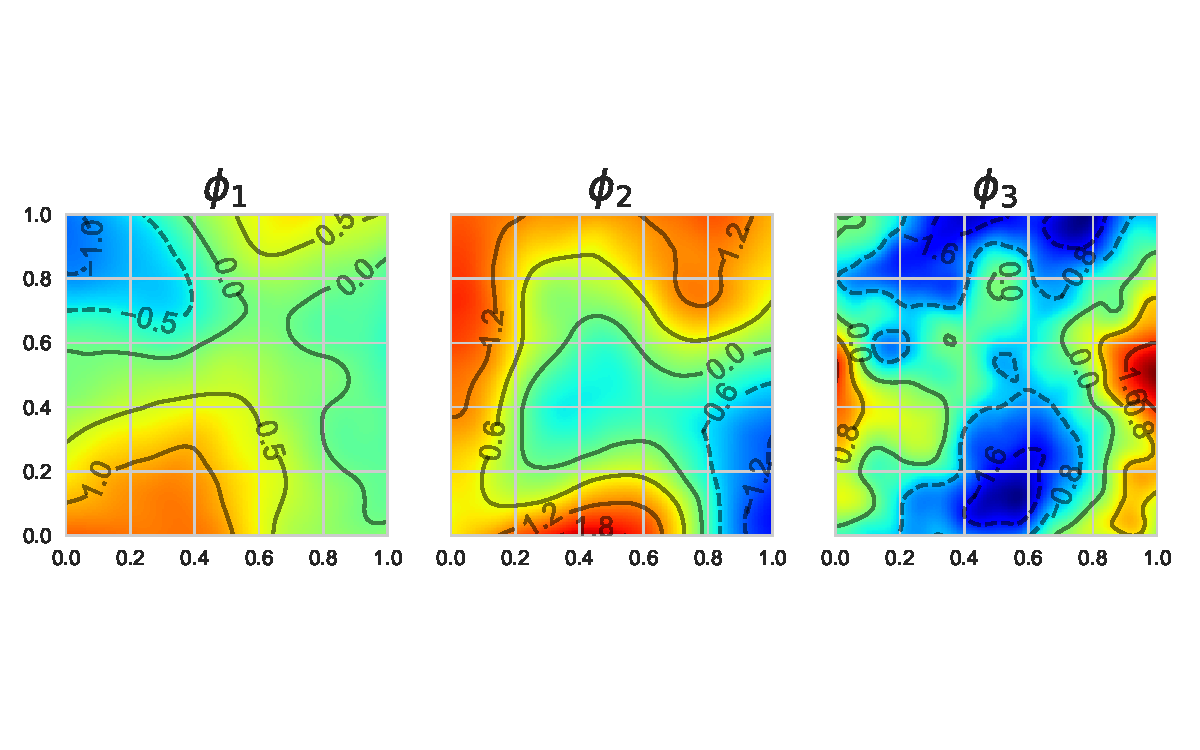
\includegraphics[width=1.0\textwidth]{sim_fpc_example}
	\caption[An example of the simulated functional principle components.]{Example of the 3 simulated principal component surfaces from the isotropic stationary Mat\`{e}rn covariance function. Notice the reduced spatial correlation in succeeding components. The simulation study is designed this way to provide difficulty for recovering the true functional principal components. }
	\label{fig:ftsm_example_fpc}
\end{figure}

To simulate the three corresponding score processes we let the variance and length scale parameters vary with component.
These hyper parameters are given in Table~\ref{tab:zeta_params}.
Again we choose these parameters to emphasise the smoothness  and contribution of the leading components to the whole processes.
That is the succeeding score processes are more variable, becoming more difficult to distinguish and forecast. 

\begin{table}[htbp!] 
	\caption[Parameters for simulating functional principal component score processes.]{The varying length scale and noise parameters in the Gaussian covariance function which is used to simulate the $3$ functional principal component scores in the data generating process.}
	\centering
	\label{tab:zeta_params}
	\begin{tabular}{l c c }
		\toprule
		& \multicolumn{2}{c}{Parameter} \\ 
		Component  & $\sigma$ &$\rho$ \\
		\midrule
		1 & 1.0 & 0.5 \\
		2 & 0.8 & 0.3 \\
		3 & 0.5 & 0.1 \\
		\bottomrule
	\end{tabular}
\end{table}

An example of the $3$ functional principal component score processes is given in Figure~\ref{fig:ftsm_example_zeta}. 
This highlights the decreasing correlation and the impact of the variance parameter on the score processes. 

\begin{figure}[htbp!] 
	\centering    
	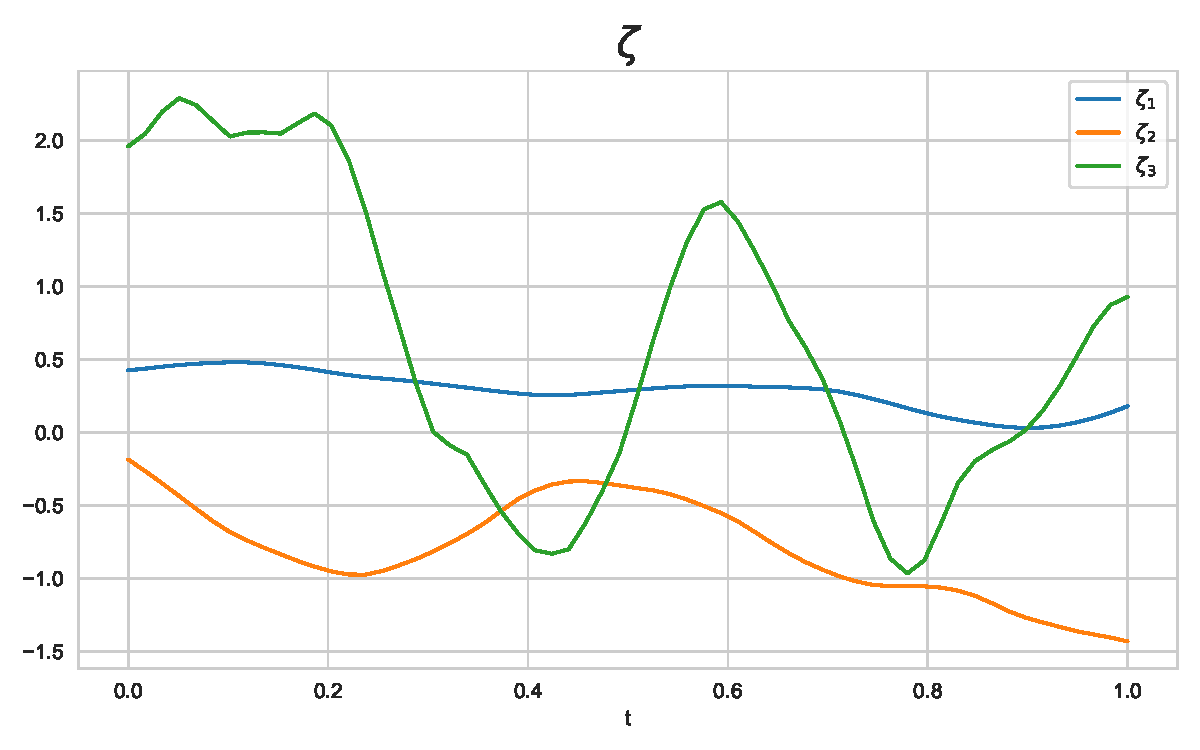
\includegraphics[width=1.0\textwidth]{sim_zeta_example}
	\caption[An example of the simulated functional principle component scores.]{Example of the 3 simulated principal component score functions from the stationary Mat\`{e}rn covariance function. Notice the reduced temporal correlation in succeeding components. The simulation study is designed this way to provide difficulty for interpolation and forecasting such components. }
	\label{fig:ftsm_example_zeta}
\end{figure}

Combining the simulated principal components with their appropriate weightings given by the simulated principal component scores then gives us a simulation from a truncated version of the model given in Equation~\eqref{eqn:space_fpca}.
Figure~\ref{fig:ftsm_chi_example} displays a selection of time points of the corresponding functional variable simulations from the components and scores displayed in Figures~\ref{fig:ftsm_example_fpc},~\ref{fig:ftsm_example_zeta} respectively. 

\begin{figure}
	\centering
	\begin{subfigure}[b]{0.45\textwidth}
		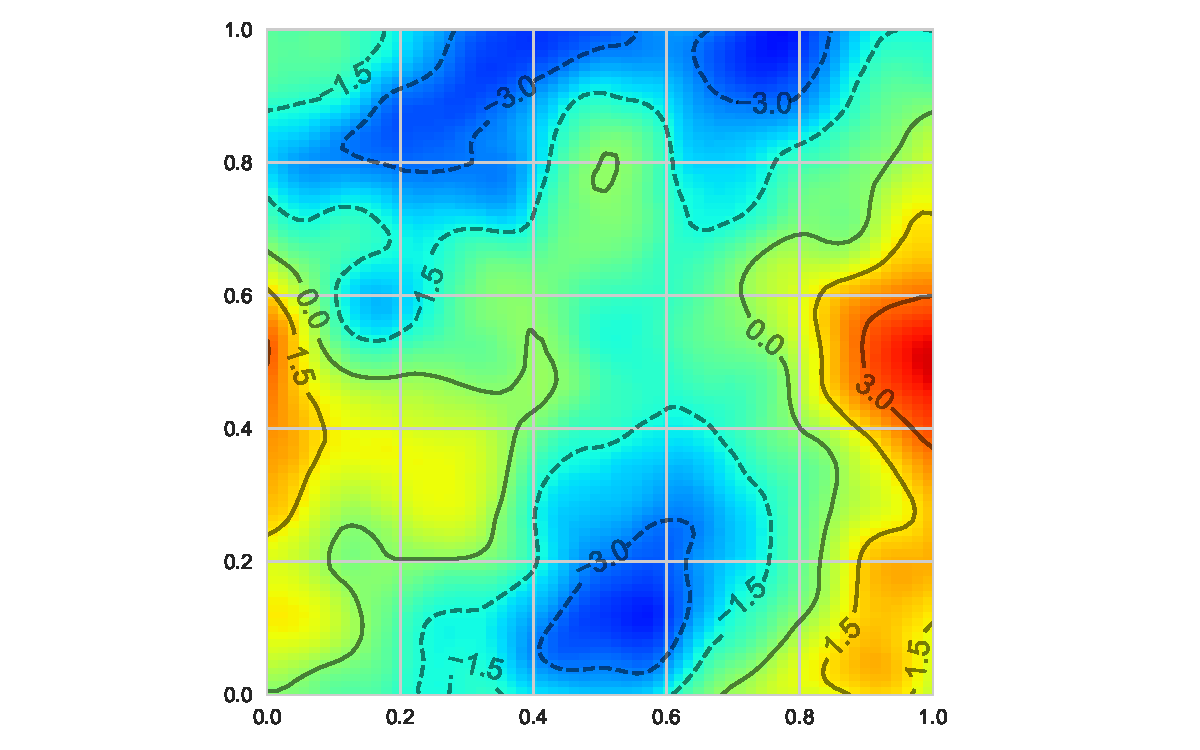
\includegraphics[width=\textwidth]{sim_chi_example_001}
		\caption{$t=0.00$}
		\label{fig:ftsm_chi_example_0}
	\end{subfigure}             
	\begin{subfigure}[b]{0.45\textwidth}
		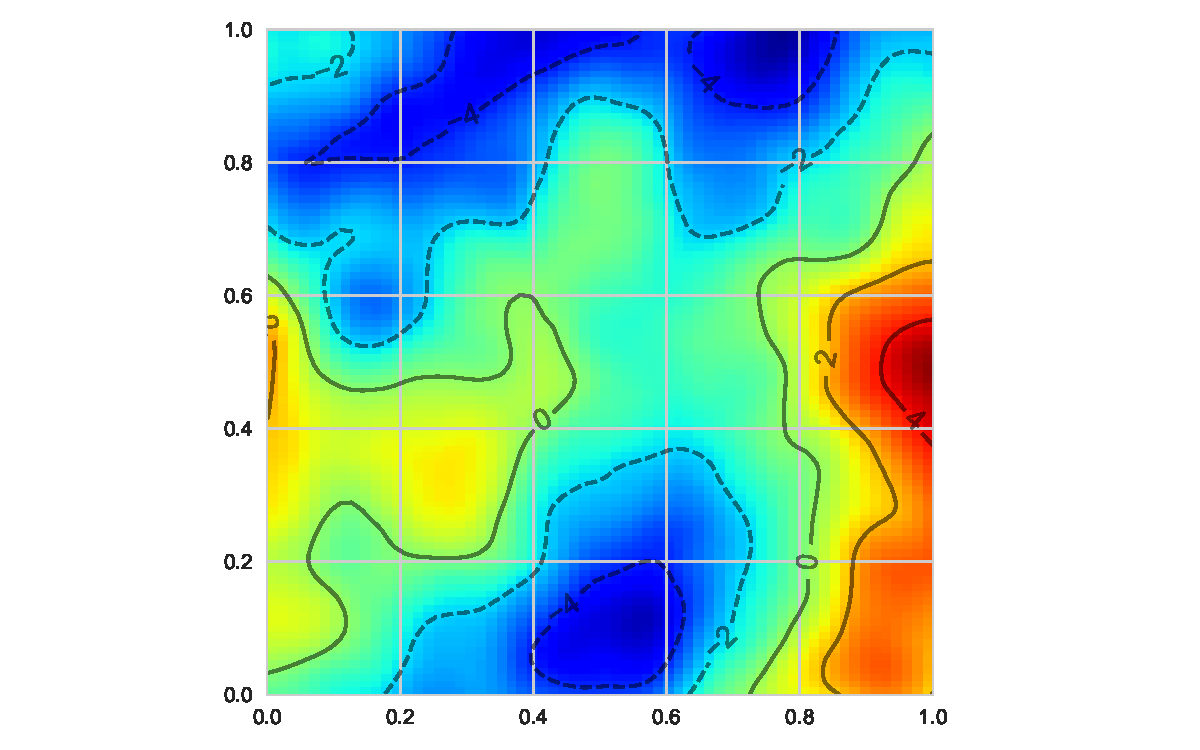
\includegraphics[width=\textwidth]{sim_chi_example_002}
		\caption{$t=0.17$}
	\end{subfigure}
	\vfill       
	\begin{subfigure}[b]{0.45\textwidth}
		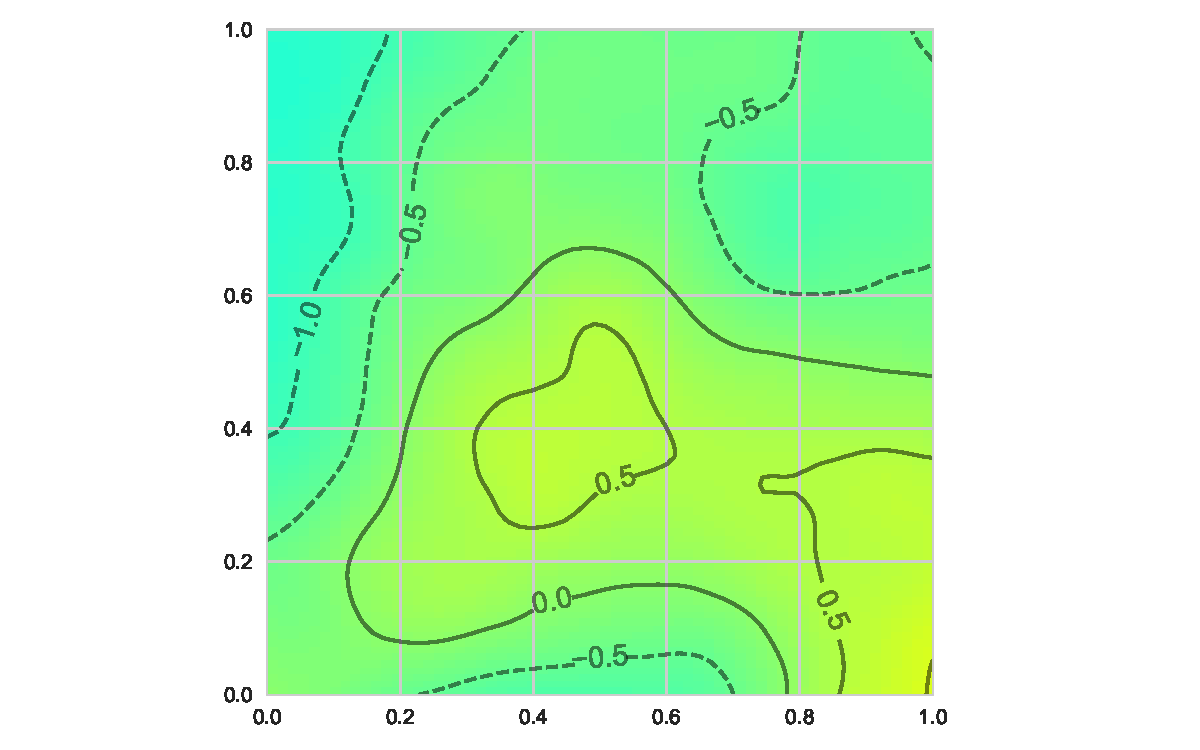
\includegraphics[width=\textwidth]{sim_chi_example_003}
		\caption{$t=0.34$}
	\end{subfigure}
	\begin{subfigure}[b]{0.45\textwidth}
		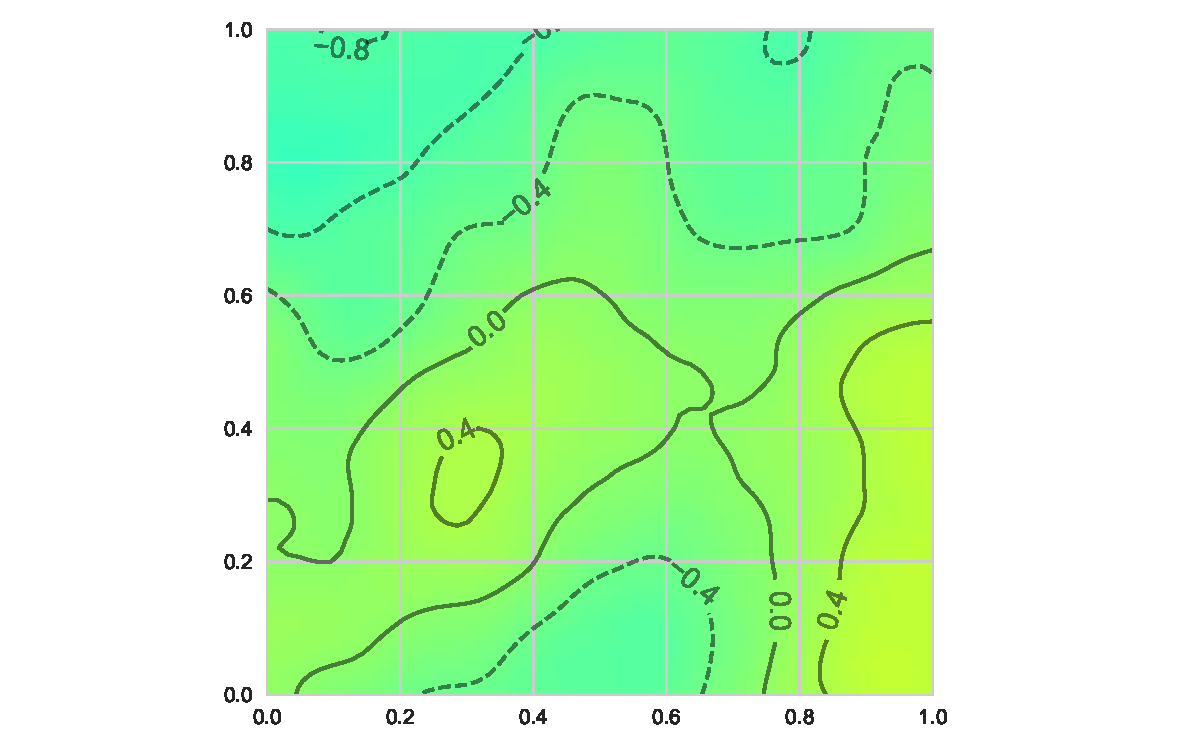
\includegraphics[width=\textwidth]{sim_chi_example_004}
		\caption{$t=0.51$}
	\end{subfigure}  
	\vfill           
	\begin{subfigure}[b]{0.45\textwidth}
		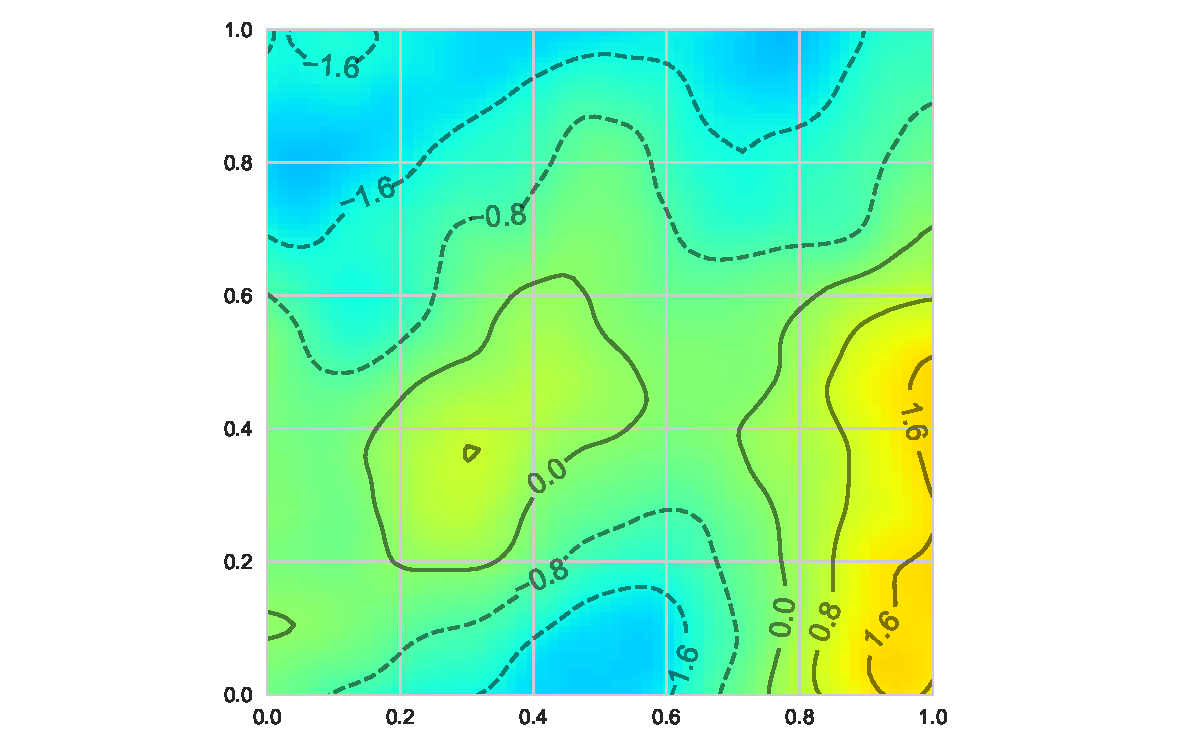
\includegraphics[width=\textwidth]{sim_chi_example_005}
		\caption{$t=0.68$}
	\end{subfigure}             
	\begin{subfigure}[b]{0.45\textwidth}
		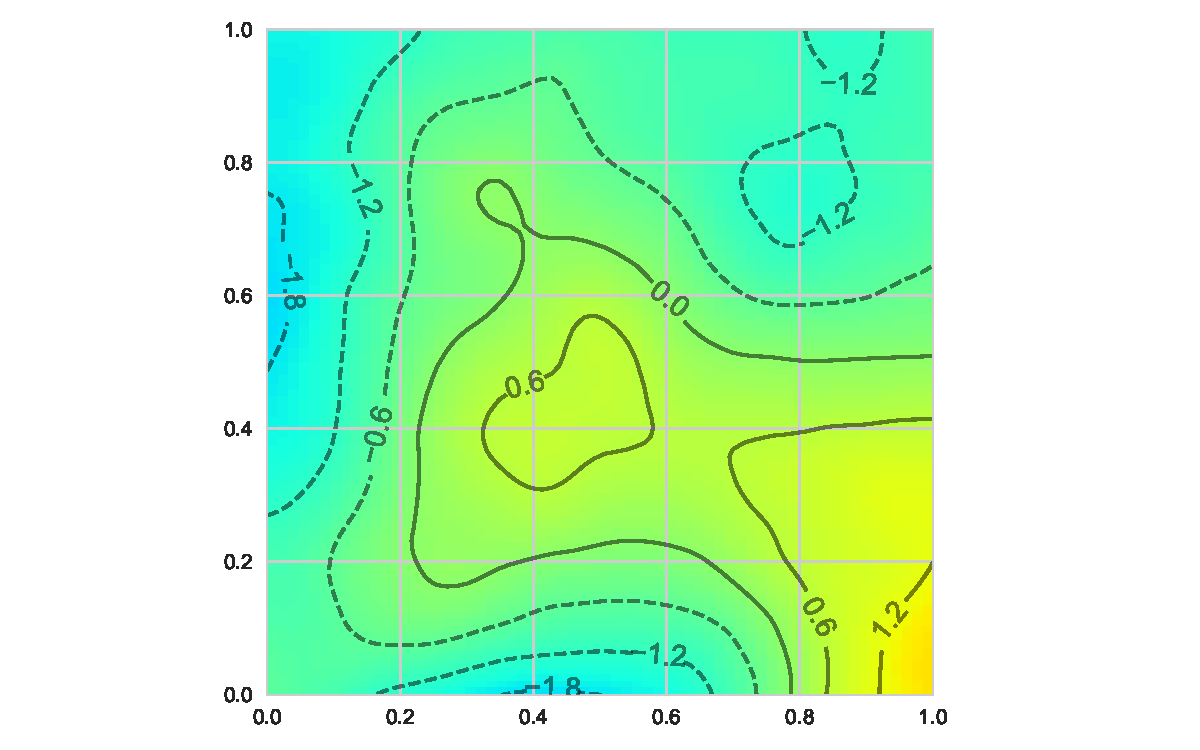
\includegraphics[width=\textwidth]{sim_chi_example_006}
		\caption{$t=0.85$}
	\end{subfigure}
	\caption[An example simulated functional variables at various times.]{An example simulated functional variables, $\bar{\chi}_j$. for various time points, $t_j$. These correspond to the simulated functional components and scores in Figures~\ref{fig:ftsm_example_fpc},~\ref{fig:ftsm_example_zeta} respectively. Notice how we see the third principal component prominently at the beginning then fade and reappear in line with its associated score, whereas the first two components are more consistent over time.}
	\label{fig:ftsm_chi_example}
\end{figure}

As given in Equation~\eqref{eqn:space_obs} we do not observe the simulated functional variable directly but rather with an additive noise process $\bar{\varepsilon_{ij}}$ for $i=1,2,\cdots, N$, $j=1,2,\cdots, J$.
For our simulation experiments we will consider 4 different types of observational noise; low variance independent noise (LN), high variance independent noise (HN), low variance isotropic spatially correlated noise with short range (LSN), and low variance isotropic spatially correlated noise with long range (HSN).
In all cases we assume the noise process is independent over time. 
We consider the first two (LN and HS) as corresponding to experiments to discuss how the model deals with typical measurement error. 
The second two noise models (LSN and HSN) correspond to an additional challenge to our models by testing their ability to recover the imagery even when there is spatially correlated noise which may look similar to that of a single functional variable. 
This is of special importance in some EO data, such as satellite imagery, where often noise corresponds to atmospheric interference which is spatially correlated, \citep{oliver_understanding_2004}. 
We consider two cases where the range of the spatial correlation changes, between short range in the LSN noise and long range
 dependency in the HSN noise. 
In these two noise process they correspond to the noise process being spatially similar to the last and first functional principal component respectively.
 In both case we simulate the noise process using a Gaussian process with zero mean and  Mat\`{e}rn covariance function. 
 We modulate the smoothness of the spatially dependent noise processes by modifying  the length scale parameter of the generating covariance function.
 Table~\ref{tab:ftsm_sim_noise_params} displays the noise process variance and shape parameters where applicable. 
 
\begin{table}[htbp!] 
	\caption[Parameters for simulating the noise process.]{Variance, length scale and structure parameters for the four different simulated noise processes. Independent noise over space corresponds to a blank $\nu$ and $\rho$ parameters. }
	\centering
	\label{tab:ftsm_sim_noise_params}
	\begin{tabular}{l c c  c}
		\toprule
		& \multicolumn{3}{c}{Parameter} \\ 
		Noise Type & $\sigma$ & $\rho$& $\nu$ \\
		\midrule
		LN & 0.2 & - & - \\
		HN & 1.0 & - & -\\
		LSN & 0.2 & 0.2 & 2.5 \\
		HSN & 0.2 & 0.5 & 2.5 \\
		\bottomrule
	\end{tabular}
\end{table}

The impact of such noise can be see in Figure~\ref{fig:ftsm_noise_example} which displays the imagery observed after adding the various noise types to the unobserved functional variable displayed in Figure~\ref{fig:ftsm_chi_example_0}. 

\begin{figure}
	\centering
	\begin{subfigure}[b]{0.45\textwidth}
		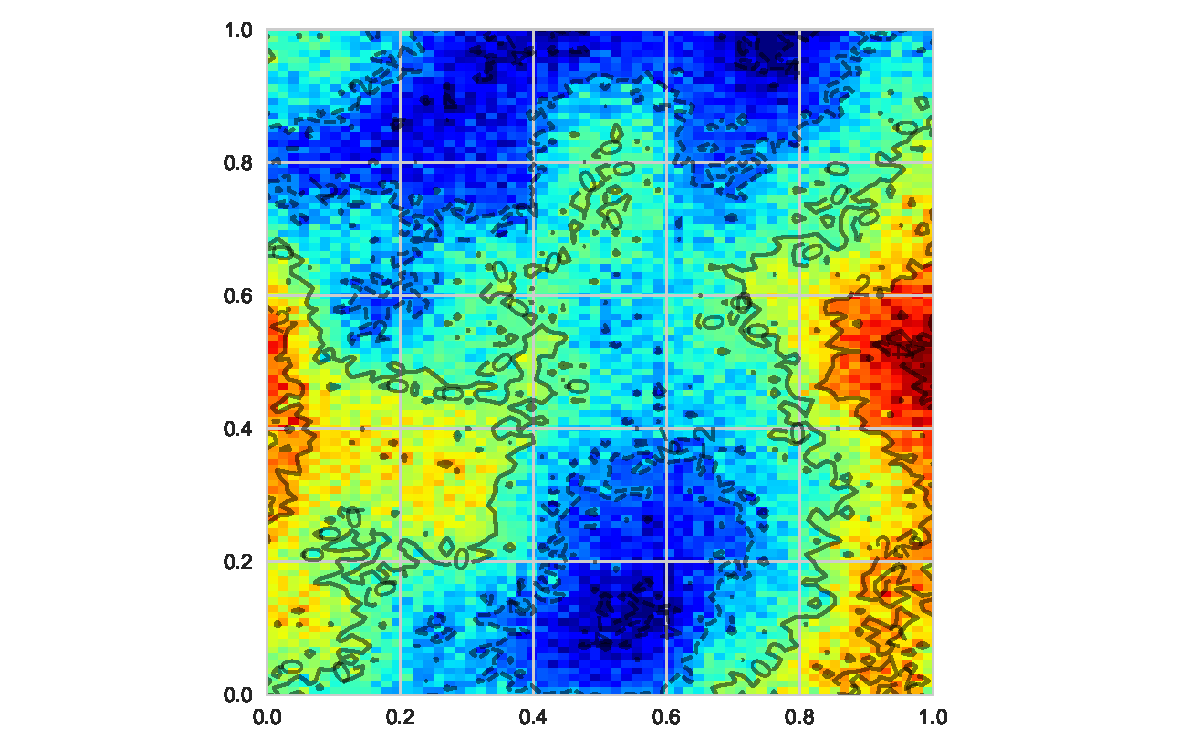
\includegraphics[width=\textwidth]{sim_noise_example_lin}
		\caption{$LN$}
		\label{fig:ftsm_noise_example_0}
	\end{subfigure}             
	\begin{subfigure}[b]{0.45\textwidth}
		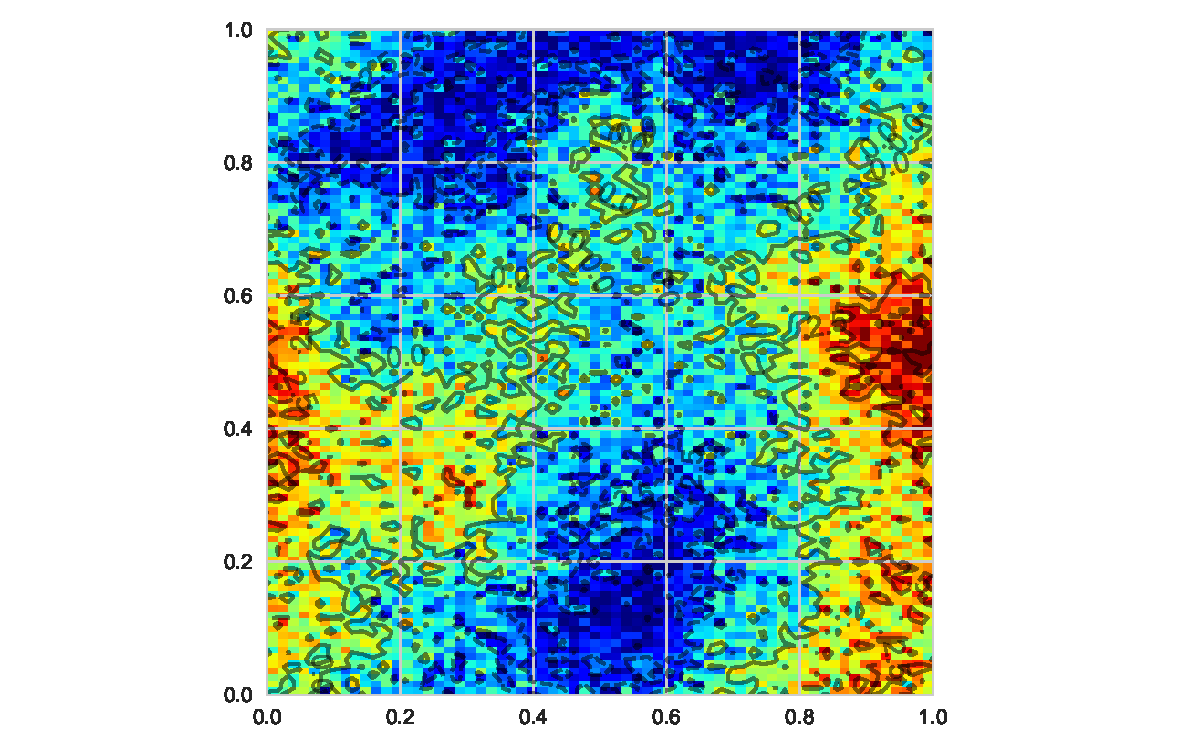
\includegraphics[width=\textwidth]{sim_noise_example_hin}
		\caption{$HN$}
	\end{subfigure}
	\vfill       
	\begin{subfigure}[b]{0.45\textwidth}
		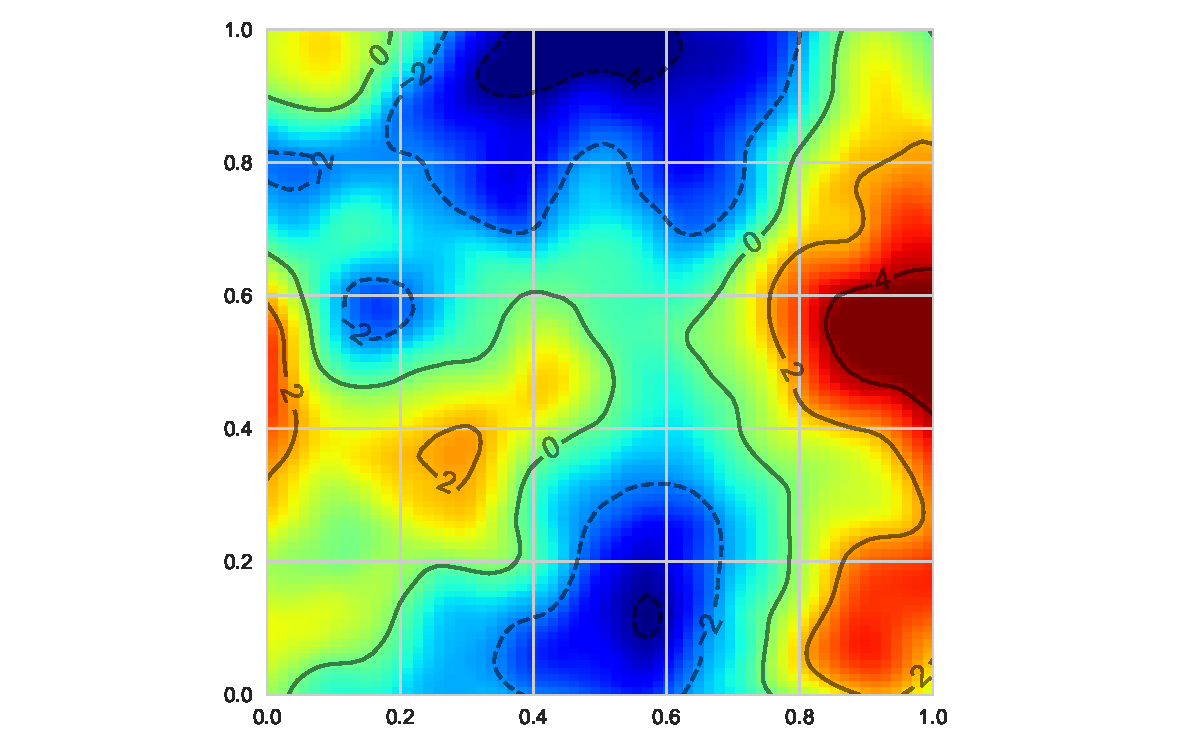
\includegraphics[width=\textwidth]{sim_noise_example_lsn}
		\caption{$LSN$}
	\end{subfigure}
	\begin{subfigure}[b]{0.45\textwidth}
		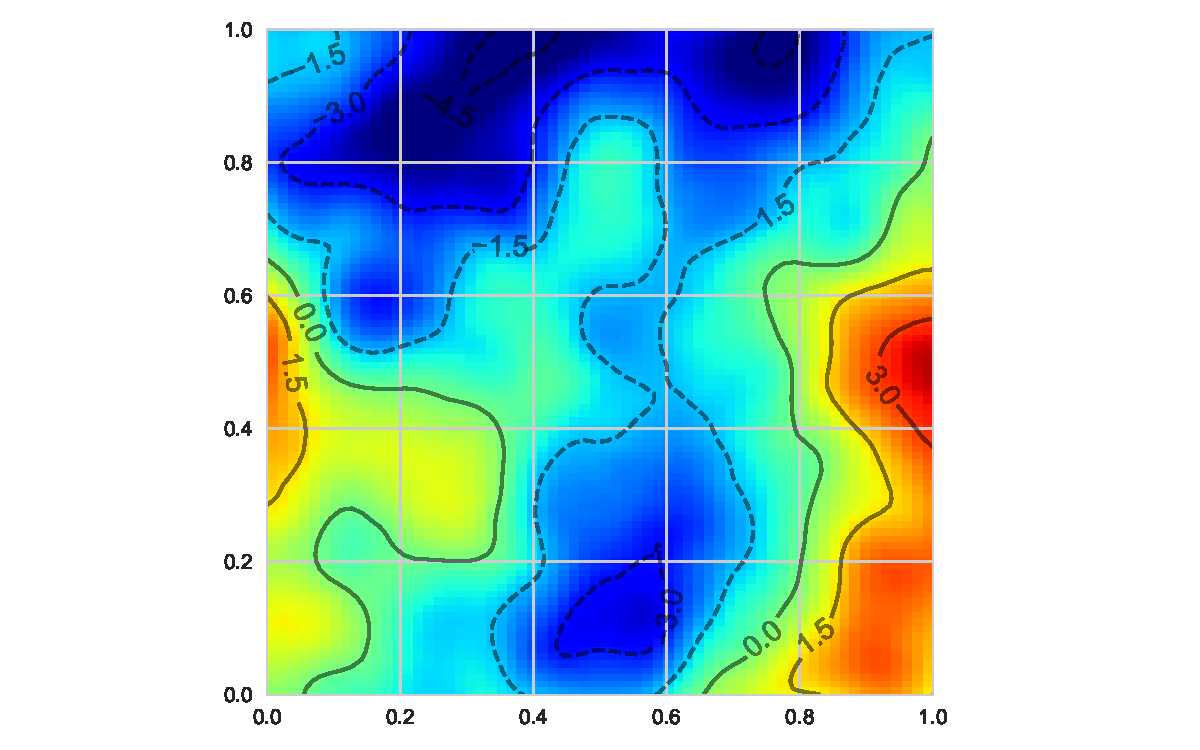
\includegraphics[width=\textwidth]{sim_noise_example_hsn}
		\caption{$HSN$}
	\end{subfigure}  
	\caption[An example of the impact of noise to observed simulated data.]{An example of the impact of the various noise structures to the observed simulated data. Each figure highlights adding a noise process to the unobserved functional variable displayed in Figure~\ref{fig:ftsm_chi_example_0}.}
	\label{fig:ftsm_noise_example}
\end{figure}

\subsection{Model parameters \label{ssec:sim_params}}
The model described in Section~\ref{sec:ftsm_model} has various hyper-parameters which control exactly how the model acts.
We specify these  below, along with justification for such choices where needed.

The first set of hyper-parameters correspond to those of the basis system used for the basis expansion of the functional variables.
In our case we limit ourselves to B-spline basis systems of order $4$, as described in Section~\ref{ssec:basis_splines}.
We choose order $4$ B-spline functions as cubic functions are the standard in many applications, \citep{de_boor_practical_2001}. 
We choose $16$ basis functions across each dimension of our surfaces, giving a total number of $256$ basis functions for the tensor product basis system, as described in Section~\ref{ssec:spline_reg}. 
This is chosen as a trade off between flexibility to fit the surface and computational constraints. 
Obviously the higher number of basis functions the closer we can recreate the observed data, however the additional computational cost in estimating these coefficients quickly grows as the number of basis functions in each dimension is increased.
To penalise the fitting, as described in Section~\ref{ssec:spline_reg}, we use the GCV fitting procedure given in \citep{wahba_spline_1990} with the tensor product penalty given by \citep{wood_p-splines_2017}.
We choose the penalty order to be $1$ which essentially places first derivative smoothness over the marginal basis, again such a choice is standard in spline fitting. 

The next set of hyper-parameters relates to the functional decomposition.
We choose to examine a maximum of $4$ principal components in our decomposition.
That is we set $K = 4$. 
This is chosen as to be a fairly substantive dimensionality reduction whilst maintaining a degree representativeness as we know through our simulation that the first $3$ components should capture the majority of the variation.
Next we set our MAFR operator $L$ to be the first order derivative.
This will again set out preference for smooth surfaces. 
Again the first order derivative is chosen as it is often a standard in functional data analysis, \citep{ramsay_functional_2010}. 

We have already stated we choose the hyper-parameters to these processes by maximum likelihood estimation of the Gaussian process.
This estimation process is discussed in detail in \citep{williams_gaussian_2006}.

The final set of simulation hyper-parameters refers to how we split between training and testing data.
The training and test data split depends on our objective of either interpolation or forecasting.
For interpolation we randomly select $30$ points of our time domain $\mathcal{T}$ as training points and observe the noisy simulated data at these points.
The remaining time points then represent the test data which we will evaluate our model performance against.
For forecasting we split the time domain at the $54^\text{th}$ time point.
Any observation before this point becomes our training data with any point after being the test data which we will forecast for. 
This gives a possibility of testing long range forecasting whilst maintaining enough training data to possibly infer patterns using the score process models.

\subsection{Results \label{ssec:ftsm_sim_res}}
We present the results for interpolation and forecasting the simulated data in this section separately, as they correspond to two separate objectives.
We repeat the simulation $100$ times for both interpolation and forecasting.
The simulation results are presented separately for each of our proposed models named FPCA and MAFR.
The details of such models are described in Section~\ref{sec:ftsm_model} and the references within.

As a comparison to these methods we use a traditional PACE model using time as our functional variable.
The details of the PACE approach are set out in Section~\ref{sec:pace}.

This is a typical model for such data.
For example, \cite{hooker_maximal_2016} uses such an approach on a similar styled data set. 
However, this approach completely ignores any spatial dependency by instead treating each pixel as independent.
Interpolation and forecasting using this methodology is performed by interpolating and extrapolating the spline basis functions in the model in standard ways, \citep{de_boor_practical_2001}.
Therefore it is mainly tailored towards interpolation as spline regression is well known to interpolate well but extrapolate poorly, \citep{de_boor_practical_2001}.
We will denote this model by the term PACE for the following results. 


To compare these models we use four metrics. 
We use two standard measure of mean square error (RMSE) and mean absolute error (MAE).
These two are chosen to contrast the influence of any particularly large discrepancies between reconstruction and actual functional variables. 
The next metric we use is the structure similarity index (SSIM), \citep{wang_image_2004}.
The SSIM metric introduced by \citeauthor{wang_image_2004} in \citeyear{wang_image_2004} and enhanced in \citeyear{wang_mean_2009} considers the case that standard metrics such as RMSE and MAE are not indicative of perceived similarity.
For example taking a grey-scale image and adding a constant value to the whole image will increase its RMSE and MAE however to the observer the image will only look brighter. 
SSIM tries to incorporate structural similarity when comparing imagery to highlight perceived similarity, \citep{wang_mean_2009}. 
The SSIM metric is calculated over various windows of an image.
The SSIM between two windows x and y of common size is given by:

\begin{equation}
	\text{SSIM}\left(x, y\right) = \frac{(2 \mu_x \mu_y + c_1)(2\sigma_{xy} + c_2)}{(\mu_x^2 + \mu_y^2 + c_1)(\sigma_x^2 + \sigma_y^2 + c_2)}
\end{equation}
where $\mu_x, \mu_y$ are the respective means of the windows, $\sigma_x, \sigma_y$ are the respective standard deviation of the windows, $\sigma_{xy}$ is the covariance of $x$ and $y$, and $c_1, c_2$ are two constants which are calculated based on the dynamic range of the two images under comparison.
For further details we refer the reader to \citep{wang_mean_2009}.
For the SSIM metric a value of $1$ represents perfect similarity, the value of $-1$ represent perfect negative similarity, hence the closer to $1$ the better for this metric.
The final metric we employ is the Peak Signal to Noise Ratio (PSNR). 
PSNR is commonly used to quantify image reconstruction quality. 
It has been used extensively in medical imaging applications.
The metric is commonly defined using the MSE between images two images $x$ and $y$ say.
Then the value is given by:
\begin{equation}
	\text{PSNR}(x, y) = 10 \log_{10}\left(\frac{\text{MAX}^2_x}{MSE(x,y)}\right)
\end{equation}
where $\text{MAX}_x$ is the maximum possible value in image $x$, and $MSE(x,y)$ is the mean square error between $x$ and $y$.  
For the PSNR metric a higher value is better. 

\subsubsection{Interpolation results}
Here we present the metric results for interpolation across our test data set as described in Section~\ref{ssec:sim_params}.
The results given are the metric value across all unobserved functional variables in the test set which we have interpolated.
We present both the average across simulations as well as the standard deviation of the metric values across simulations.

Tables~\ref{tab:ftsm_sim_interp} displays the reconstruction results for interpolation from the various observations with the different noise processes structures. 
Discussion of these results can be found in Section~\ref{ssec:ftsm_sim_disc}. 

\begin{table}[htbp!] 
	\caption[Simulation results for interpolation by noise scenario with the three models under consideration.]{Simulation results for interpolation by noise scenario for each model; PACE, FPCA, and MAFR. Bracketed values correspond to the standard deviation. Bold values illustrate best in class.}
	\centering
	\label{tab:ftsm_sim_interp}
	\begin{tabular}{l l c c c c}
		\toprule
		& & \multicolumn{4}{c}{Metric} \\ 
		Noise & Model & RMSE & MAE & SSIM & PSNR \\
		\midrule
		\multirow{3}{*}{LN}& PACE & 0.25 (0.05) & 0.20 (0.04) & 0.80 (0.07) & 28.15 (3.37) \\
		& FPCA  & \textbf{0.10 (0.05)} & \textbf{0.08 (0.04)} & \textbf{0.98 (0.02)} & \textbf{35.27 (4.59)} \\
		& MAFR  & 0.12 (0.10) & 0.10 (0.08) & 0.97 (0.02)  & 34.66 (5.08) \\
		\midrule
		\multirow{3}{*}{HN} & PACE & 0.40 (0.06) & 0.32 (0.05) & 0.58 (0.09) & 24.26 (2.93) \\
		& FPCA  & \textbf{0.16 (0.05)} & \textbf{0.13 (0.04)} & \textbf{0.95 (0.03)} & \textbf{31.78 (4.23)} \\
		& MAFR  & 0.19 (0.07) & 0.15 (0.06) & 0.94 (0.03)  & 31.06 (4.30) \\
		\midrule
		\multirow{3}{*}{LSN} & PACE & 0.50 (0.08) & 0.41 (0.07) & 0.88 (0.04) & 23.49 (2.59) \\
		& FPCA  & \textbf{0.46 (0.07)} & \textbf{0.38 (0.06)} & \textbf{0.88 (0.05)} & \textbf{23.56 (2.77)} \\
		& MAFR  & 0.48 (0.08) & 0.39 (0.06) & \textbf{0.88 (0.05)}  & 23.45 (2.56)\\
		\midrule
		\multirow{3}{*}{HSN} & PACE & 0.50 (0.10) & 0.42 (0.09) & \textbf{0.93 (0.04)} & \textbf{23.65 (3.12)}  \\
		& FPCA  & 0.51 (0.10) & 0.42 (0.09) & 0.90 (0.05) & 22.61 (2.72) \\
		& MAFR  & \textbf{0.48 (0.10)} & \textbf{0.40 (0.09)} & 0.92 (0.04) & 23.61 (2.71) \\
		\bottomrule
	\end{tabular}
\end{table}

\subsubsection{Forecasting results}
Here we present the metric results for the forecasting ability of our models for our test data set as described in Section~\ref{ssec:sim_params}.
The results given are the metric value at $h$-step ahead forecasts for the unobserved functional variables in the test set where $h$ is one of $1, 3, 6$.
A single step ahead corresponds to observing the next image on our temporal grid $\mathcal{T}$ constructed in our data generating process. 
These correspond loosely to short, medium, and long range forecasts. 
This provides an overview of the abilities of the model to forecast over various ranges.
These $h$ step ahead comparisons are standard in time series forecasting, \citep{hyndman_forecasting_2021}. 
We present both the average across simulations as well as the standard deviation of the metric values across simulations.

Tables~\ref{tab:ftsm_sim_for} displays the reconstruction results for each model in our simulation studies under our forecasting scenario. 
Discussion of these results can be found in Section~\ref{ssec:ftsm_sim_disc}. 

\begin{landscape}
\begin{table}
	\caption[Simulation results for forecasting by noise scenario with the three models under consideration.]{Simulation results for the models ability to forecast unseen functional variables under the FTSM model at $1, 3, 6$ time steps ahead. Bracketed values correspond to the standard deviation. Bold values illustrate best in class.}
	\centering
		
	\label{tab:ftsm_sim_for}
	\resizebox{1.6\textwidth}{!}{\begin{tabular}{l l c c c c c c c c c c c c}
		\toprule
		& & \multicolumn{12}{c}{Metric} \\ 
		 & & \multicolumn{3}{c}{RMSE} &  \multicolumn{3}{c}{MAE} &  \multicolumn{3}{c}{SSIM} &  \multicolumn{3}{c}{PSNR} \\
		Noise & Model & $h=1$ & $h=3$ & $h=6$ & $h=1$ & $h=3$ & $h=6$ & $h=1$ & $h=3$ & $h=6$ & $h=1$ & $h=3$ & $h=6$\\
		\midrule
		\multirow{3}{*}{LN} & PACE & 0.35 (0.12) & 0.68 (0.27) & 1.14 (0.49)) & 0.28 (0.09) & 0.54 (0.22) & 0.92 (0.40) & 0.60 (0.14) & 0.41 (0.17) & 0.29 (0.19) & 20.21 (3.60) & 19.18 (2.98) & 17.28 (4.03)  \\
		& FPCA  & 0.10 (0.05) & 0.28 (0.17) & \textbf{0.59 (0.33)} & \textbf{0.08 (0.04)} & 0.23 (0.14) & \textbf{0.48 (0.27)} & \textbf{0.94 (0.06)} & \textbf{0.90 (0.14)} & \textbf{0.74 (0.27)} & \textbf{28.42 (7.01)} & \textbf{25.72 (5.97)} & \textbf{20.38 (6.07)} \\
		& MAFR  & \textbf{0.10 (0.05)} & \textbf{0.28 (0.16)} & 0.60 (0.36) & \textbf{0.08 (0.04)} & \textbf{0.23 (0.13)} & 0.49 (0.29) & \textbf{0.94 (0.06)} & 0.88 (0.15) & 0.73 (0.27) & 28.04 (6.46) & 25.39 (5.60) & 20.21 (5.74) \\
		\midrule
		\multirow{3}{*}{HN} & PACE& 0.53 (0.18) & 0.90 (0.35) & 1.36 (0.54) & 0.43 (0.14) & 0.72 (0.28) & 1.09 (0.43) & 0.44 (0.11) & 0.29 (0.12) & 0.19 (0.13)  & 18.37 (2.76) & 17.62 (2.36) & 16.17 (3.28) \\
		& FPCA  & \textbf{0.17 (0.08)} & \textbf{0.34 (0.19)} & \textbf{0.63 (0.32)} & \textbf{0.14 (0.06)} & \textbf{0.28 (0.16)} & \textbf{0.52 (0.27)} & \textbf{0.90 (0.11)} & \textbf{0.86 (0.15)} & \textbf{0.72 (0.27)} & \textbf{25.62 (5.60)} & \textbf{23.81 (5.34)} & \textbf{19.47 (5.58)}  \\
		& MAFR  & \textbf{0.17 (0.08)} & 0.36 (0.19) & 0.69 (0.37) & 0.14 (0.07) & 0.29 (0.15) & 0.57 (0.31) & 0.88 (0.12) & 0.83 (0.17) & 0.70 (0.25) & 24.72 (5.61) & 22.64 (4.88) & 18.68 (5.42)  \\
		\midrule
		\multirow{3}{*}{LSN} & PACE & 0.74 (0.26) & 1.21 (0.49) & 1.72 (0.64) & 0.61 (0.22) & 1.00 (0.42) & 1.42 (0.54) & 0.76 (0.13) & 0.63 (0.19) & 0.47 (0.26)  & 18.37 (3.28) & 16.54 (3.21) & 14.12 (3.57) \\
		& FPCA  & \textbf{0.54 (0.24)} & \textbf{0.70 (0.35)} & \textbf{0.90 (0.45)} & \textbf{0.44 (0.19)} & \textbf{0.58 (0.28)} & \textbf{0.74 (0.38)} & 0.77 (0.20) & 0.70 (0.25) & 0.59 (0.31) & \textbf{19.86 (4.72)} & \textbf{18.52 (4.56)} & \textbf{16.53 (4.96)}  \\
		& MAFR  & 0.56 (0.20) & 0.74 (0.30) & 0.97 (0.44) & 0.47 (0.16) & 0.61 (0.25) & 0.80 (0.37) & \textbf{0.78 (0.17)} & \textbf{0.72 (0.21)} & \textbf{0.61 (0.28)} & 19.54 (4.32) & 18.29 (4.21) & 16.22 (4.42) \\
		\midrule
		\multirow{3}{*}{HSN} & PACE & 0.74 (0.29) & 1.21 (0.47) & 1.71 (0.68) & 0.62 (0.25) & 1.01 (0.42) & 1.43 (0.60) & \textbf{0.82 (0.13)} & 0.70 (0.21) & 0.54 (0.32) & 18.45 (3.34) & 17.01 (3.37) & 14.86 (4.17)  \\
		& FPCA  & 0.60 (0.23) & 0.75 (0.34) & \textbf{0.94 (0.46)} & 0.50 (0.19) & \textbf{0.62 (0.29)} & \textbf{0.78 (0.39)} & 0.79 (0.20) & \textbf{0.74 (0.22)} & 0.62 (0.29) & 19.87 (4.97) & 18.83 (4.89) & 16.43 (4.75)  \\
		& MAFR  & \textbf{0.59 (0.24)} & \textbf{0.75 (0.33)} & 0.97 (0.46) & \textbf{0.49 (0.21)} & 0.63 (0.28) & 0.81 (0.40) & 0.82 (0.17) & 0.76 (0.21) & \textbf{0.64 (0.30)}  & \textbf{20.22 (4.83)} & \textbf{18.98 (4.66)} & \textbf{16.65 (4.85)} \\
		\bottomrule
	\end{tabular}}
\end{table}
\end{landscape}

\subsection{Discussion \label{ssec:ftsm_sim_disc}}

We discuss the preceding results for the FPCA and MAFR models in the following section.
We discuss the results relative to the PACE model as described in Section~\ref{ssec:ftsm_sim_res} under both the interpolation and forecasting objectives.

Table~\ref{tab:ftsm_sim_interp} states the mean and standard deviations of the estimation error under the various metrics discussed in Section~\ref{ssec:ftsm_sim_res} for the interpolation metric.
We can see clearly an advantage of using the FPCA model over the PACE model under most metrics in nearly all noise process scenarios.
The only exception to this being under the highly structured spatial noise process, denoted by HSN, where the FPCA model is inferior to the MAFR and PACE models; though only slightly.
This advantage is most prominent under the independent noise scenarios where it seems that the additional spatial smoothness constraints that the model enforces nullifies the impact of the spatially independent noise.
Similarly, the relative deterioration in the FPCA model under structured noise agrees with this effect.
In fact it is possible that due to the noise process being highly similar to the leading functional principal components in the HSN scenario that the FPCA model may conflate the two, hence giving reduced performance.

The MAFR model has similar performance to that of the FPCA model; as expected, due to it being a rotated version of the FPCA model.
It is narrowly but consistently beaten on most noise scenarios, except for the HSN.
Here, the fact that the MAFR model prioritises smoothness in its components, \citep{hooker_maximal_2016}, has meant that we have overcome some of the trouble that the FPCA model faced of conflating the noise and signal processes. 
We can see this effect by examining the second functional principal component for both the FPCA and MAFR model for a single simulation under the HSN noise scenario as an example.
Figure~\ref{fig:ftsm_res_example_fpc} shows exactly this.
The actual functional principal components for this simulation are given in Figure~\ref{fig:ftsm_example_fpc}.

\begin{figure}[!htbp]
	\centering
	\begin{subfigure}[b]{0.45\textwidth}
		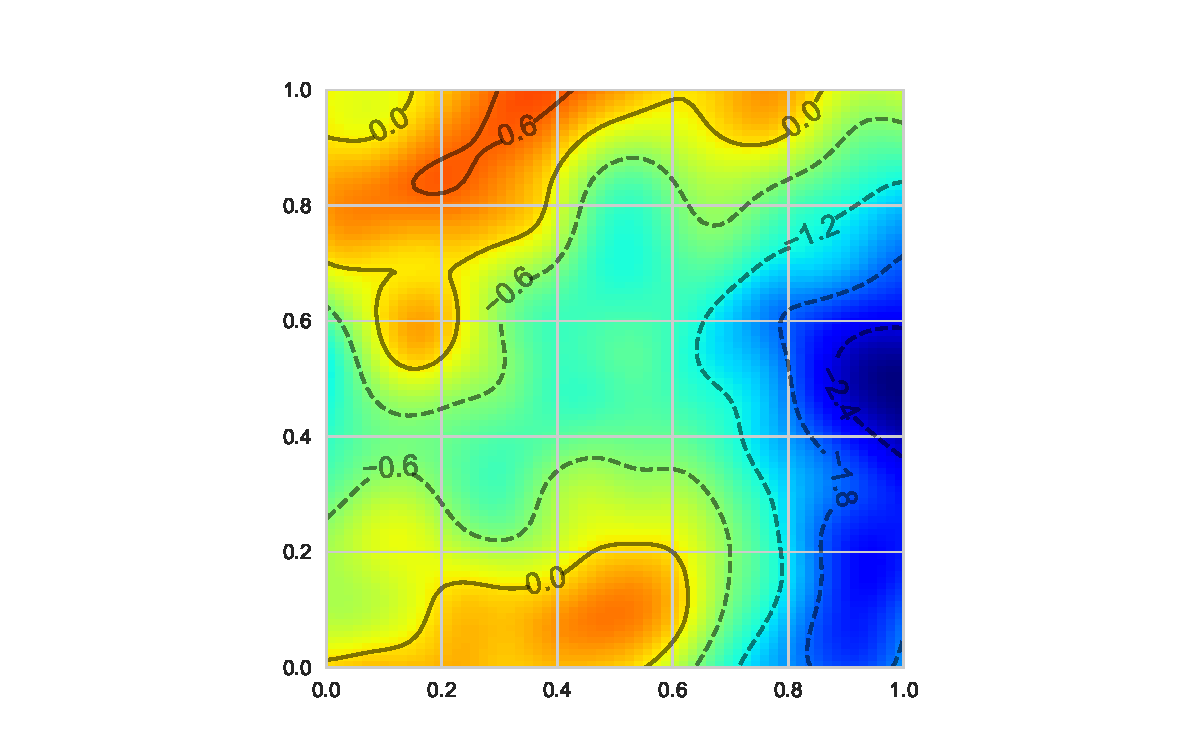
\includegraphics[width=\textwidth]{ftsm_res_fpc_example_fpca}
		\caption{FPCA}
	\end{subfigure}             
	\begin{subfigure}[b]{0.45\textwidth}
		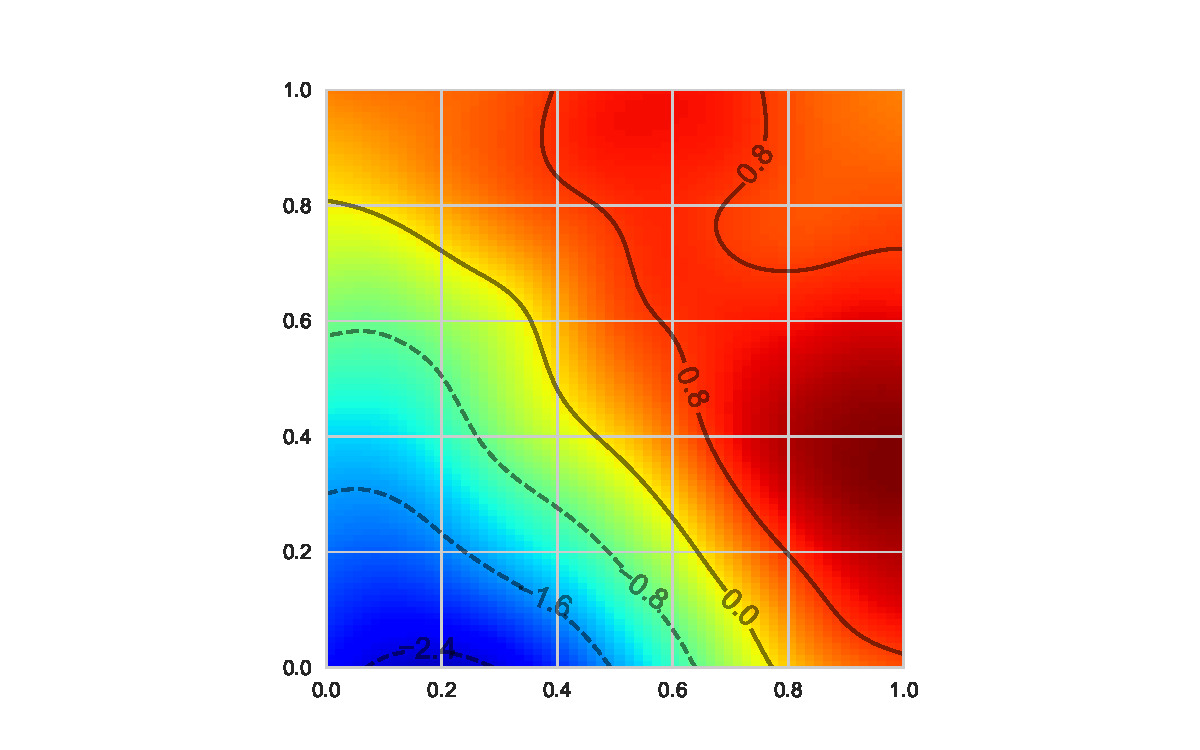
\includegraphics[width=\textwidth]{ftsm_res_fpc_example_mafr}
		\caption{MAFR}
	\end{subfigure}
	\caption[Comparison of the second functional principal component under FPCA and MAFR models.]{Comparison of the second functional principal component recovered under the FPCA model and the MAFR model for an example simulation under the HSN noise scenario. Notice how the MAFR component is much smoother over the domain.}
	\label{fig:ftsm_res_example_fpc}
\end{figure}

In addition, this rotation has caused the score processes to be correlated to the point that leading components will have smoother scores, aiding in removing the noise process which will have random walk like behaviour in the scores process due to it being independent over time.
This is illustrated in Figure~\ref{fig:ftsm_res_example_zeta} where we can see that although both score processes aren't particularly smooth the MAFR process exhibits less variation. 

\begin{figure}[htbp!] 
	\centering    
	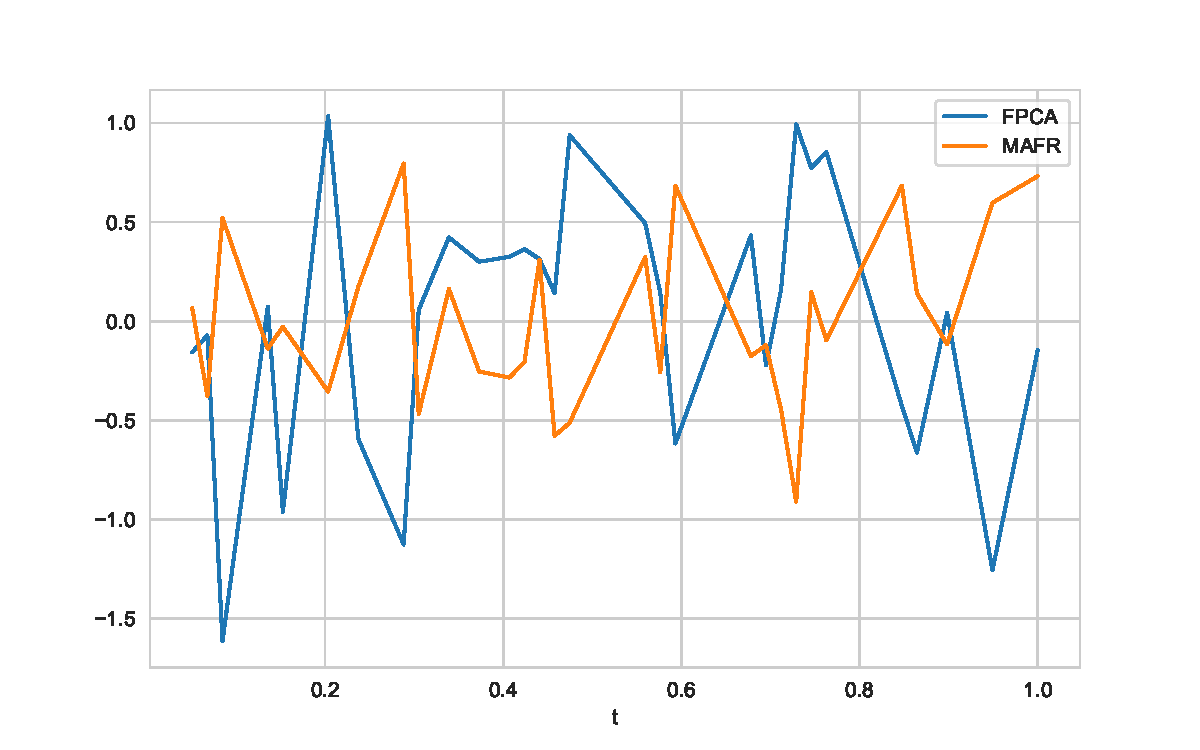
\includegraphics[width=1.0\textwidth]{ftsm_res_zeta_example}
	\caption[Comparison of the second score process under FPCA and MAFR models.]{Comparison of the second score process corresponding to the second functional principal component given in Figure~\ref{fig:ftsm_res_example_fpc}. Notice how the MAFR score process exhibits less variation over time compared to the FPCA process.}
	\label{fig:ftsm_res_example_zeta}
\end{figure}

The result for the forecasting objective are given in Table~\ref{tab:ftsm_sim_for}.
Here, we see similar results to that which were observed in the interpolation objective.
We see both the FPCA and MAFR models outperform the PACE model under most noise scenarios.
Similarly to the interpolation results we see the most improvement under spatially independent noise processes.
Again, this is due to the added ability of the FPCA and MAFR models to filter out any process which isn't particularly smooth over space. 
Interestingly, we also see a greater improvement in reconstruction for the long term forecast rather than the one step ahead short term forecast relative to the PACE model.
This is good as it suggests that the FPCA and MAFR approaches capture the spatio-temporal process in such a way that is easier to forecast. 
Figure~\ref{fig:ftsm_res_recon} highlights this ability by illustrating the unobserved surface and estimated surfaces for each model under the LN noise scenario at three time steps ahead.

\begin{figure}
	\centering
	\begin{subfigure}[b]{0.45\textwidth}
		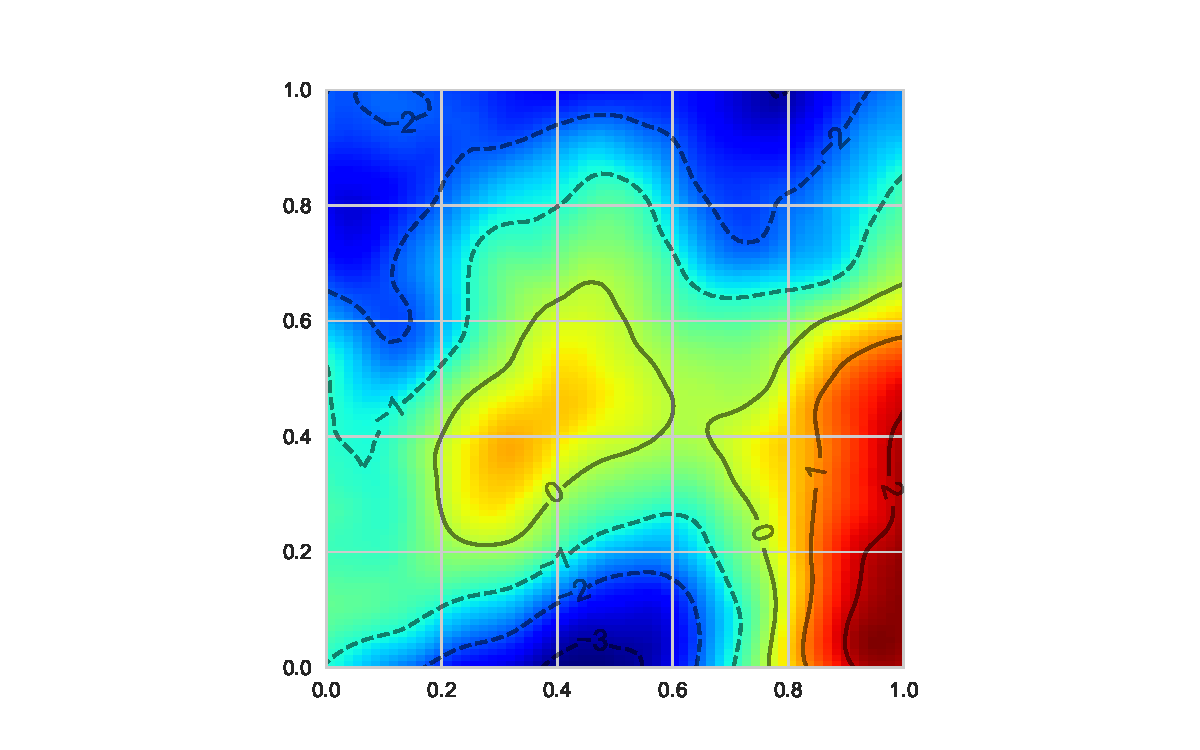
\includegraphics[width=\textwidth]{ftsm_res_recon_example_unob}
		\caption{$Unobserved$}
		\label{fig:ftsm_res_recon_unob}
	\end{subfigure}             
	\begin{subfigure}[b]{0.45\textwidth}
		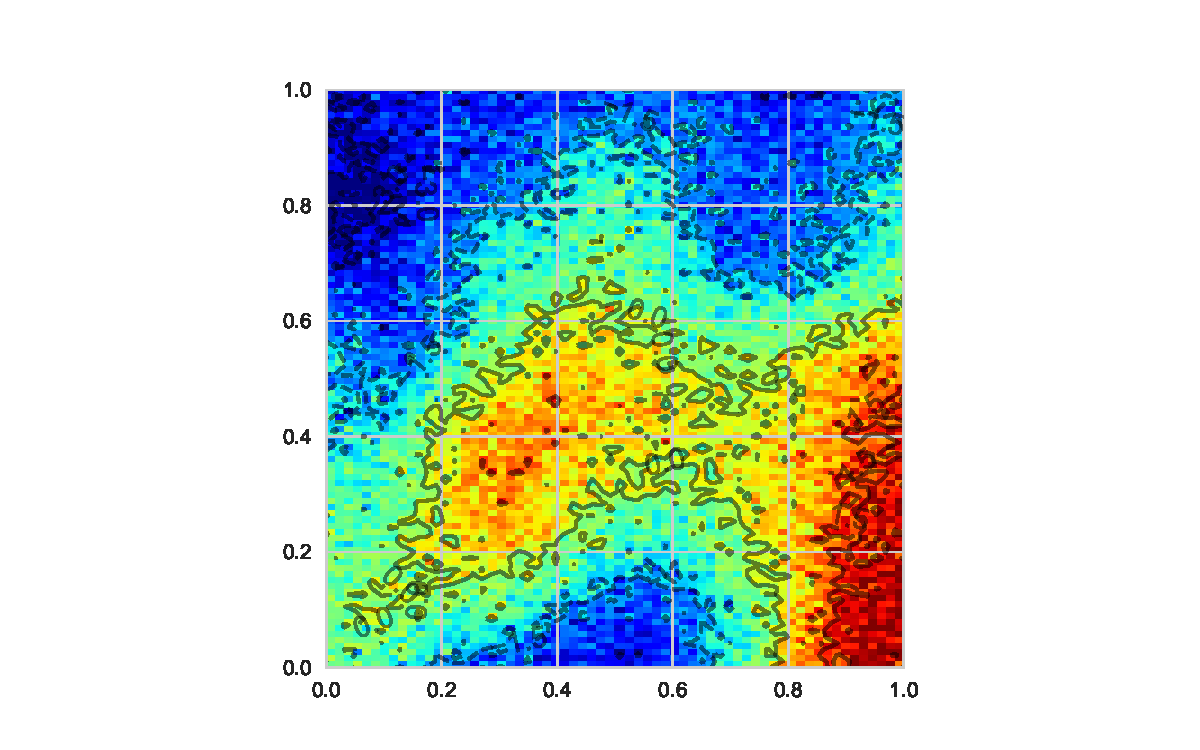
\includegraphics[width=\textwidth]{ftsm_res_recon_example_pace}
		\caption{$PACE$}
		\label{fig:ftsm_res_recon_pace}
	\end{subfigure}
	\vfill       
	\begin{subfigure}[b]{0.45\textwidth}
		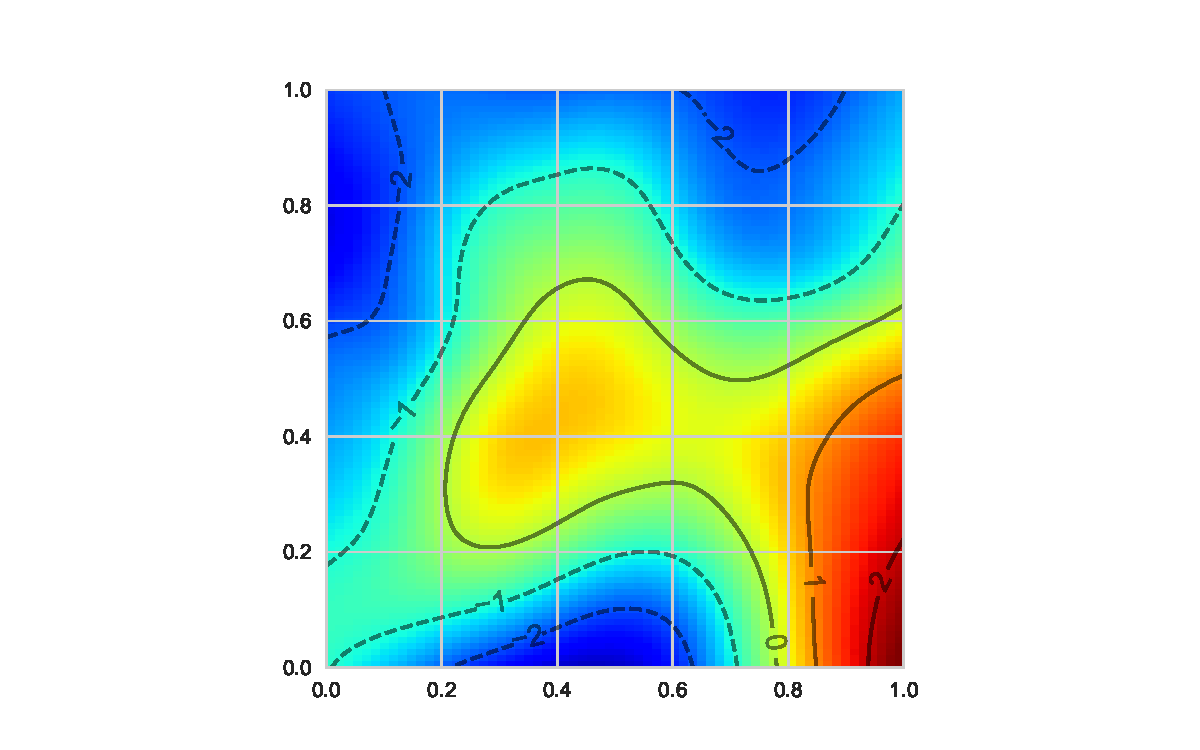
\includegraphics[width=\textwidth]{ftsm_res_recon_example_fpca}
		\caption{$FPCA$}
		\label{fig:ftsm_res_recon_fpca}
	\end{subfigure}
	\begin{subfigure}[b]{0.45\textwidth}
		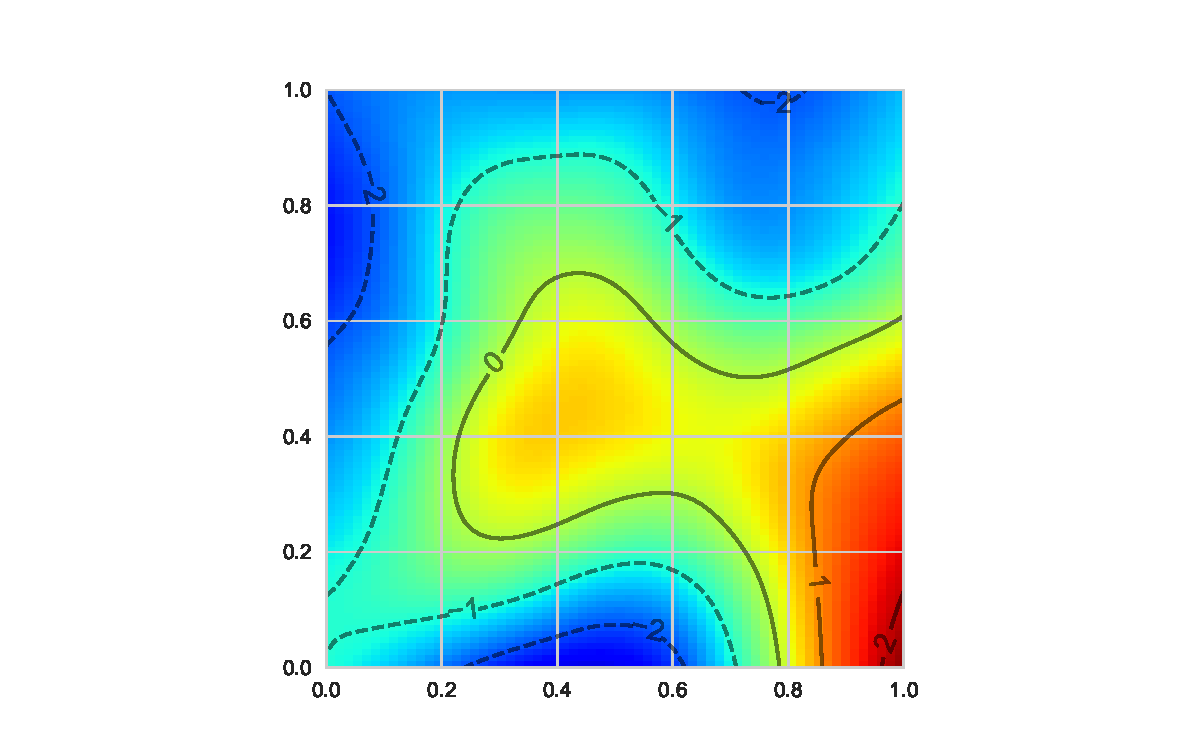
\includegraphics[width=\textwidth]{ftsm_res_recon_example_mafr}
		\caption{$MAFR$}
		\label{fig:ftsm_res_recon_mafr}
	\end{subfigure}  
	\caption[Example of the impact of the various models to reconstruct the unobserved surface at three steps ahead.]{Example of the impact of the various models to reconstruct the unobserved surface at three steps ahead. The observed process was corrupted by the LN noise process. We note how the PACE model is easily over fitting to the independent noise process whereas the FPCA and MAFR models do not suffer this effect.}
	\label{fig:ftsm_res_recon}
\end{figure}

Again the FPCA and MAFR approaches result in similar results, with the FPCA model edging the results for the majority of the noise processes.
Similarly to the interpolation results we see that the MAFR model tends to perform better under the HSN noise scenario. 
This is due to the same reasons as the interpolation results described above. 

These results offer a good indication that including spatial information into the model for such data sets can have a material impact on both interpolating and forecasting objectives. 
The next test for such models is then to see how this improvement translates to data sets not necessarily coming from the data generating procedure.
We consider this by applying these model to our EO dataset as discussed in Chapter~\ref{cha:data} in the next section. 

\section{EO Application \label{sec:ftsm_eo}}
We apply the same models as used in the simulation model to our CESM-LE data set as described in Chapter~\ref{cha:data}.
This data set acts as an example to highlight the performance of the various models described above on a real world data set. 
We perform the exact same analysis as in the simulation study but this time apply it to the $40$ replications of the CESM-LE data for the various atmospheric variable. 

We use the exact same model parameter setup as described in Section~\ref{ssec:sim_params} to setup the models for the EO application study.
We detail the results of the study in Section~\ref{ssec:ftsm_eo_res}.

\subsection{Results \label{ssec:ftsm_eo_res}}
We present the reconstruction results for the objectives of interpolation and forecasting separately. 
We repeat the model fitting and reconstruction procedure independently for the $40$ realisations of the CESM-LE data set and provide both the mean metric measures as well as their standard deviations across these realisations. 
We use the same $4$ metrics as used in the simulation study for consistency. 

\subsubsection{Interpolation results}
Here we present the metric results for interpolation for our test data set from our CESM-LE EO observations, as described in Chapter~\ref{cha:data}.
See Section~\ref{ssec:sim_params} for the construction methodology of the test and training data sets. 
The results given are the metric value across all unobserved functional variables in the test set which we have interpolated.
We present both the average across simulations as well as the standard deviation of metric values across simulations.

Table~\ref{tab:ftsm_eo_interp} displays the reconstruction results for interpolation from the various atmospheric variables.
Discussion of these results can be found in Section~\ref{ssec:ftsm_eo_disc}.

\begin{table}[htbp!] 
	\caption[Results for interpolation by atmospheric components with various FTSM models for the CESM-LE dataset.]{Results for interpolation by atmospheric components with various FTSM models for the CESM-LE dataset. Bracketed values correspond to the standard deviation.}
	\centering
	\label{tab:ftsm_eo_interp}
	\resizebox{\textwidth}{!}{\begin{tabular}{l l c c c c}
		\toprule
		& & \multicolumn{4}{c}{Metric} \\ 
		Component & Model & RMSE & MAE & SSIM & PSNR \\
		\midrule
		\multirow{3}{*}{TMQ}&PACE & \textbf{5.60 (0.52)} & \textbf{4.31 (0.47)} & \textbf{0.73 (0.05)} & \textbf{18.61 (1.49)} \\
		& FPCA  & 6.08 (0.30) & 4.56 (0.25) & 0.70 (0.01) & 18.19 (0.52) \\
		& MAFR  &6.03 (0.30) & 4.52 (0.25) & 0.70 (0.01)  & 18.39 (0.75) \\
		\midrule
		\multirow{3}{*}{PS} & PACE & \textbf{511.40 (30.69)} & \textbf{374.56 (22.04)} & \textbf{0.99 (0.00)} & \textbf{33.83 (3.35)} \\
		& FPCA  & 2976.61 (4.81) & 1814.34 (6.92) & 0.70 (0.00) & 21.50 (0.49) \\
		& MAFR  & 2977.02 (5.68) & 1815.04 (7.44) & 0.70 (0.00)  & 21.51 (0.52) \\
		\midrule
		\multirow{3}{*}{TREFHT} & PACE & \textbf{6.80 (1.05)} & \textbf{5.05 (0.84)} & \textbf{0.90 (0.02)} & \textbf{23.69 (2.58)} \\
		& FPCA  & 7.45 (0.35) & 5.33 (0.25) & 0.84 (0.00) & 20.43 (0.44) \\
		& MAFR  & 7.48 (0.47) & 5.38 (0.37) & 0.83 (0.00)  & 20.39 (0.36)\\
		\midrule
		\multirow{3}{*}{U10} & PACE & \textbf{1.25 (0.12)} & \textbf{0.92 (0.08)} & \textbf{0.76 (0.03)} & \textbf{19.27 (1.70)}  \\
		& FPCA  & 1.55 (0.03) & 1.20 (0.02) & 0.55 (0.00) & 16.33 (0.77) \\
		& MAFR  &1.55 (0.03) & 1.19 (0.02) & 0.55 (0.00) & 16.32 (0.81) \\
		\bottomrule
	\end{tabular}}
\end{table}

\subsubsection{Forecasting results}
Here we present the metric results for the forecasting ability of our models for our test data set from our CESM-LE EO observations, as described in Chapter~\ref{cha:data}.
See Section~\ref{ssec:sim_params} for the construction methodology of the test and training data sets. 
The results given are the metric value at $h$-step ahead forecasts for the unobserved functional variables in the test set where $h$ is one of $1, 3, 6$. 
These correspond to short, medium, and long range forecasts.
In the CESM-LE data set each step corresponds to a month interval.
This provides an overview of the abilities of the model to forecast over various ranges.
We present both the average across simulations as well as the standard deviation of the metric values across simulations.

Tables~\ref{tab:ftsm_eo_for} displays the reconstruction results for each model in our simulation studies under our forecasting scenario. 
Discussion of these results can be found in Section~\ref{ssec:ftsm_eo_disc}.

\begin{landscape}
	\begin{table}
		\caption[Results for forecasting by variable with various FTSM model on the CESM-LE dataset.]{Results for the models ability to forecast unseen functional variables under the FTSM models at $1, 3, 6$ time steps ahead in the CESM-LE dataset. Bracketed values correspond to the standard deviation. Bold represents best in class.}
		\centering
		\label{tab:ftsm_eo_for}
		\resizebox{1.6\textwidth}{!}{\begin{tabular}{l l c c c c c c c c c c c c}
			\toprule
			& & \multicolumn{12}{c}{Metric} \\ 
			& & \multicolumn{3}{c}{RMSE} &  \multicolumn{3}{c}{MAE} &  \multicolumn{3}{c}{SSIM} &  \multicolumn{3}{c}{PSNR} \\
			Noise & Model & $h=1$ & $h=3$ & $h=6$ & $h=1$ & $h=3$ & $h=6$ & $h=1$ & $h=3$ & $h=6$ & $h=1$ & $h=3$ & $h=6$\\
			\midrule
			\multirow{3}{*}{TMQ} & PACE & \textbf{3.50 (0.67)} & \textbf{5.92 (1.34)} & 5.81 (2.20) & \textbf{2.41 (0.54)} & \textbf{4.71 (1.04)} & 4.17 (1.72) & 0.45 (0.02) & 0.51 (0.03) & 0.39 (0.03) & 12.22 (0.50) & 13.30 (0.48) & 11.78 (0.46)  \\
			& FPCA  & 4.11 (0.46) & 9.62 (1.17) & 5.16 (0.86) & 2.71 (0.36) & 7.48 (0.99) & 3.65 (0.67) & \textbf{0.77 (0.01)} & \textbf{0.60 (0.05)} & \textbf{0.72 (0.03)} & 20.30 (0.89) & \textbf{16.27 (1.10)} & 18.96 (1.03)  \\
			& MAFR  & 4.12 (0.52) & 9.61 (1.20) & \textbf{5.12 (0.98)} & 2.75 (0.42) & 7.46 (1.02) & \textbf{3.62 (0.77)} & 0.77 (0.02) & \textbf{0.60 (0.05)} & \textbf{0.72 (0.03)} & \textbf{20.33 (0.84)} & 16.24 (1.11) & \textbf{19.00 (0.86)} \\
			\midrule
			\multirow{3}{*}{PS} & PACE & \textbf{572.92 (254.02)} & \textbf{1416.61 (3179.94)} & 4167.61 (19882.51) & \textbf{440.70 (243.79)} & \textbf{1176.94 (3209.63)} & 3919.64 (19920.73) & \textbf{0.98 (0.06)} & \textbf{0.98 (0.06)}  & \textbf{0.97 (0.07)} & \textbf{32.54 (5.30)} & \textbf{33.17 (5.42)} & \textbf{33.09 (5.88)}\\
			& FPCA  & 2963.55 (16.73) & 2962.08 (13.00) & 2967.76 (11.98) & 1801.39 (26.40) & 1800.56 (20.45) & 1810.16 (24.96) & 0.70 (0.00) & 0.70 (0.00) & 0.69 (0.00) & 20.96 (0.46) & 21.03 (0.46) & 21.16 (0.44)  \\
			& MAFR  & 2962.67 (17.11) & 2962.55 (15.21) & \textbf{2965.04 (9.17)} & 1800.63 (27.52) & 1802.48 (25.31) & \textbf{1804.88 (20.88)} & 0.70 (0.00) & 0.70 (0.00) & 0.69 (0.00) & 20.96 (0.36) & 21.03 (0.38) & 21.17 (0.35)  \\
			\midrule
			\multirow{3}{*}{TREFHT} &PACE & 10.13 (0.59) & 27.36 (1.16) & 30.60 (1.13) & 6.90 (0.36) & 18.52 (0.80) & 20.17 (0.79) & 0.81 (0.01) & \textbf{0.81 (0.01)} & 0.59 (0.01)  & 17.48 (0.54) & 18.04 (0.68) & 17.03 (0.49)  \\
			& FPCA  & \textbf{5.87 (1.31)} & \textbf{10.75 (1.66)} & \textbf{4.42 (1.05)} & \textbf{4.03 (0.89)} & \textbf{7.66 (1.28)} & \textbf{3.34 (0.83)} & \textbf{0.85 (0.02)} & 0.77 (0.03) & \textbf{0.85 (0.01)} & \textbf{21.59 (1.39)} & \textbf{18.80 (1.59)} & \textbf{21.56 (0.77)}  \\
			& MAFR  & 6.29 (1.05) & 11.30 (1.36) & 4.65 (1.18) & 4.36 (0.73) & 8.12 (1.15) & 3.56 (1.01) & 0.84 (0.01) & 0.76 (0.02) & 0.84 (0.02) & 21.19 (1.00) & 18.26 (1.15) & 21.40 (0.85) \\
			\midrule
			\multirow{3}{*}{U10} & PACE & \textbf{1.21 (0.07)} & \textbf{1.51 (0.12)} & \textbf{1.27 (0.11)} & \textbf{0.91 (0.06)} & \textbf{1.11 (0.10)} & \textbf{0.92 (0.08)} & \textbf{0.78 (0.02)} & \textbf{0.71 (0.03)} & \textbf{0.74 (0.03)} & \textbf{21.47 (0.74)} & \textbf{19.84 (0.88)} & \textbf{21.31 (0.82)}  \\
			& FPCA  & 1.43 (0.06) & 1.75 (0.11) & 1.41 (0.06) & 1.12 (0.05) & 1.34 (0.09) & 1.10 (0.05) & 0.56 (0.02) & 0.50 (0.03) & 0.56 (0.02) & 16.50 (0.83) & 16.05 (0.85) & 17.03 (0.74)  \\
			& MAFR  & 1.43 (0.05) & 1.75 (0.09) & 1.41 (0.04) & 1.12 (0.05) & 1.34 (0.08) & 1.10 (0.04) & 0.56 (0.02) & 0.49 (0.02) & 0.56 (0.02)  & 16.37 (0.61) & 15.93 (0.59) & 16.91 (0.53) \\
			\bottomrule
		\end{tabular}}
	\end{table}
\end{landscape}

\subsection{Discussion \label{ssec:ftsm_eo_disc}}
We discuss the preceding results for the FPCA and MAFR models with application on the CESM-LE data set in the following section.
We discuss the results relative to the PACE model as described in Section~\ref{ssec:ftsm_sim_res} under both the interpolation and forecasting objectives.

Evidently, from Table~\ref{tab:ftsm_eo_interp}, the PACE model outperforms both the FPCA and MAFR models for all atmospheric variables studied across all metrics.
This is particularly the case for the PS and U10 variables. 
The reason for this divergence from the PACE model can be seen by considering an example from the PS variable.
Figure~\ref{fig:ftsm_res_ps} gives the unobserved surface and the estimated surfaces from the PACE, FPCA, and MAFR models.
We can clearly see from this that the FPCA and MAFR models, although they capture large scale spatial patterns, fail to capture the small scale spatial variation.
In this case this causes very divergent results as seen by the metrics in Table~\ref{tab:ftsm_eo_interp}. 
The reason for this lack of flexibility of the FPCA and MAFR models is that the number of basis functions to represent the surface is not high enough to capture such spatial variability. 
Therefore, an obvious way to perhaps alleviate this problem is to simply increase the dimension of the spline representation of these surfaces. 
However, this comes with additional computation cost.
Another possibility is to just consider the FPCA and MAFR models on smaller sections of the domain which may vary less.
It is reassuring however to see that the FPCA and MAFR models do capture the large scale spatial variation well.
In fact, as the FPCA and MAFR metric values tend to vary less than those of the PACE model, if one is interested in large scale variation these models may well still be preferred.

 \begin{figure}
 	\centering
 	\begin{subfigure}[b]{0.45\textwidth}
 		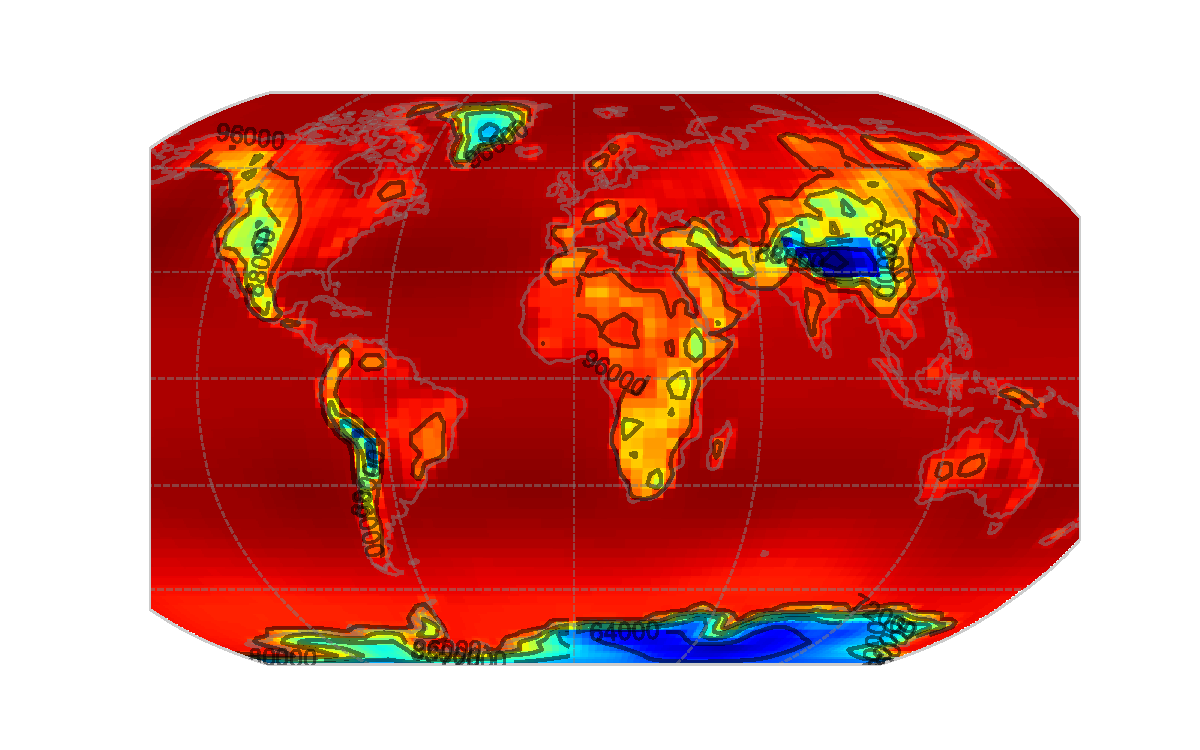
\includegraphics[width=\textwidth]{ftsm_res_ps_example_unob}
 		\caption{$Unobserved$}
 		\label{fig:ftsm_res_ps_unob}
 	\end{subfigure}             
 	\begin{subfigure}[b]{0.45\textwidth}
 		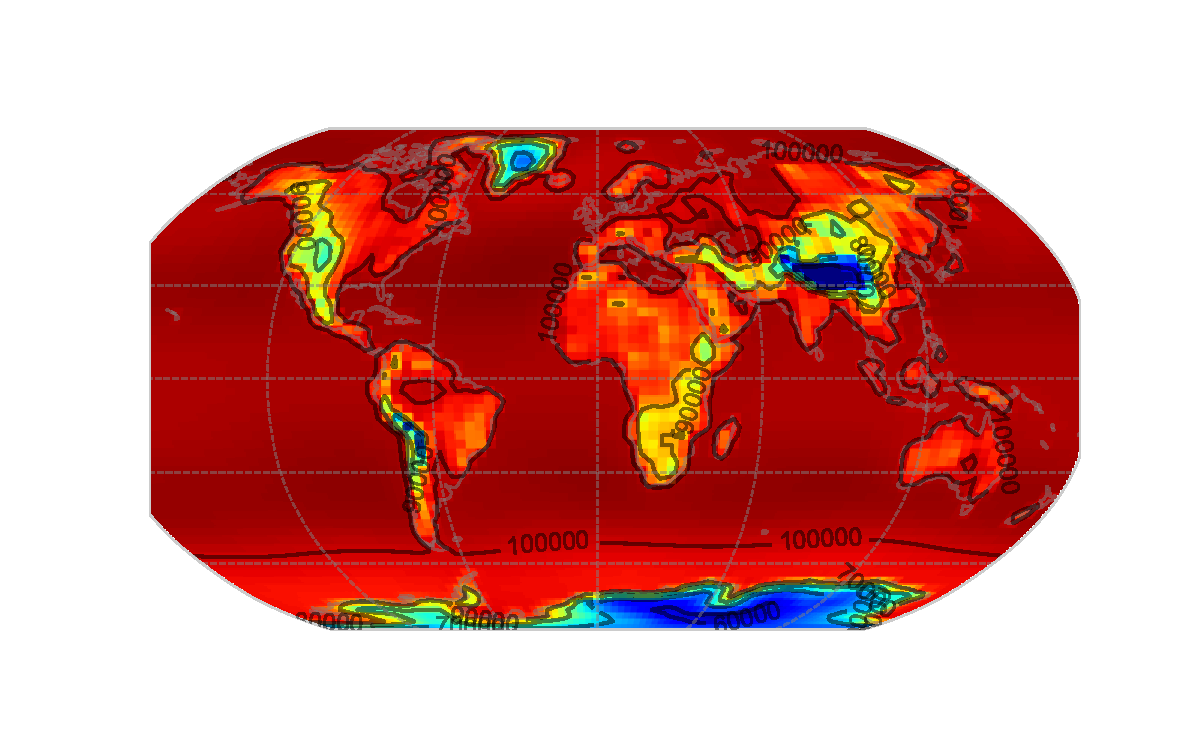
\includegraphics[width=\textwidth]{ftsm_res_ps_example_pace}
 		\caption{$PACE$}
 		\label{fig:ftsm_res_ps_pace}
 	\end{subfigure}
 	\vfill       
 	\begin{subfigure}[b]{0.45\textwidth}
 		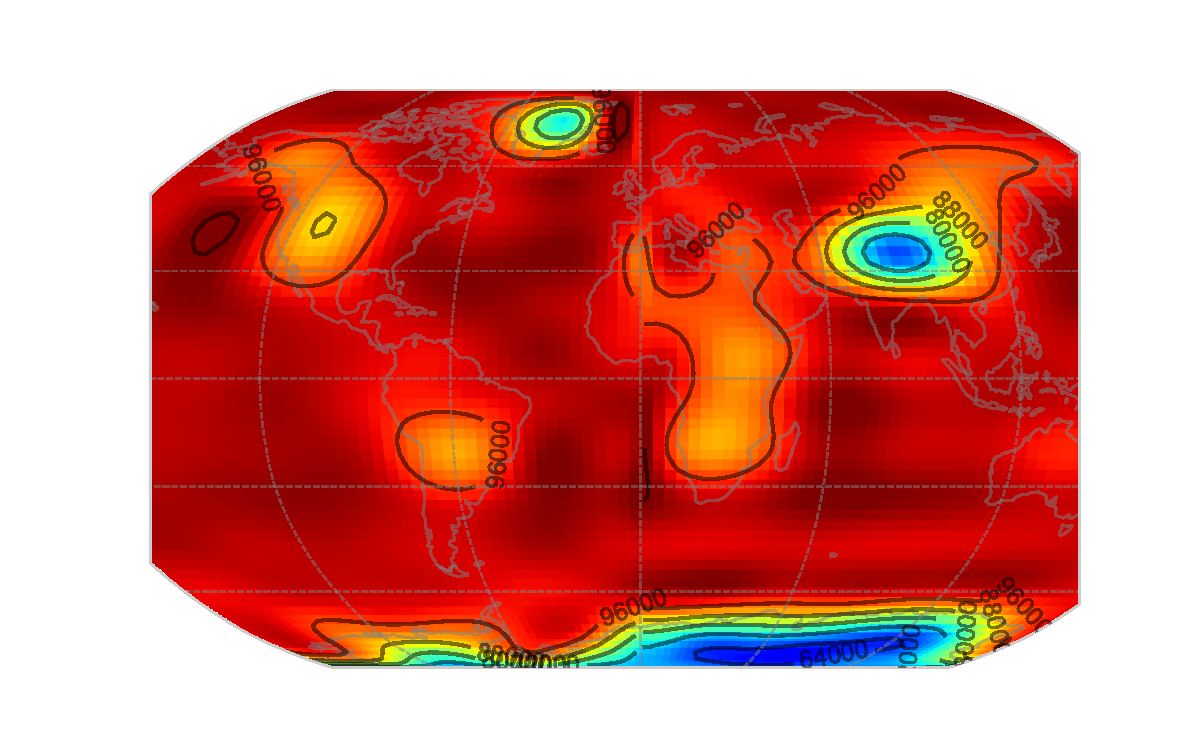
\includegraphics[width=\textwidth]{ftsm_res_ps_example_fpca}
 		\caption{$FPCA$}
 		\label{fig:ftsm_res_ps_fpca}
 	\end{subfigure}
 	\begin{subfigure}[b]{0.45\textwidth}
 		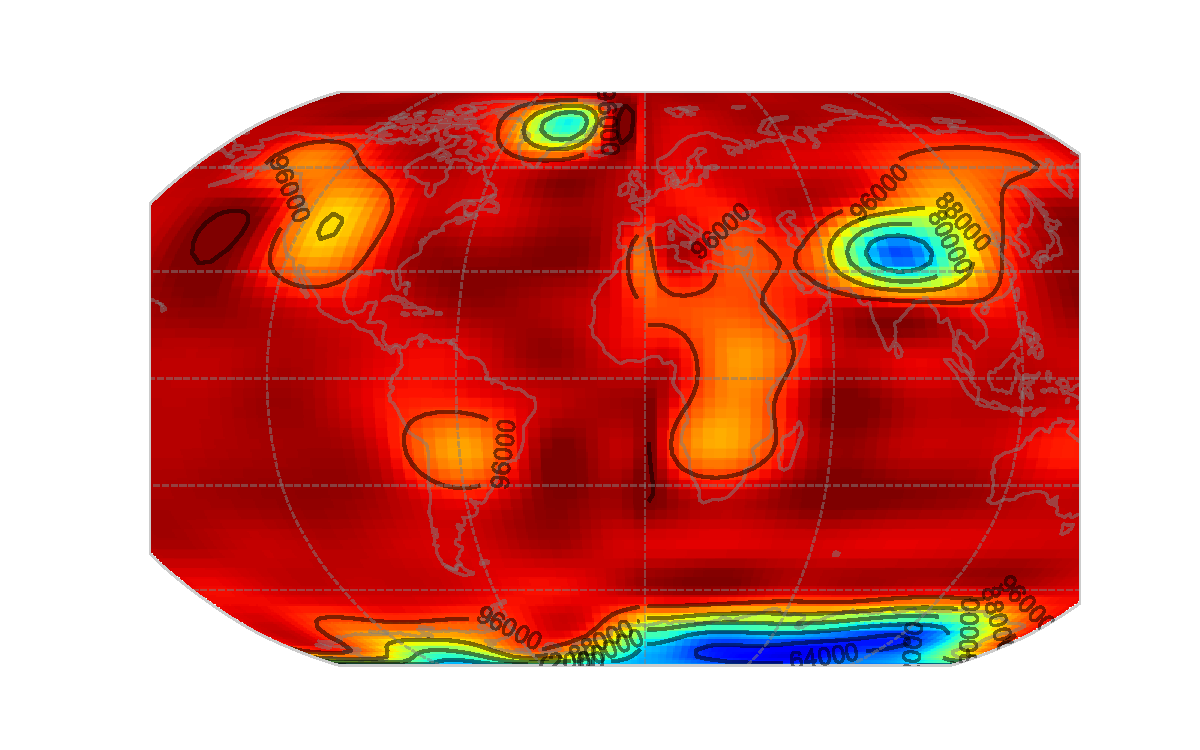
\includegraphics[width=\textwidth]{ftsm_res_ps_example_mafr}
 		\caption{$MAFR$}
 		\label{fig:ftsm_res_ps_mafr}
 	\end{subfigure}  
 	\caption[Example of the reconstruction ability of the various models for the PS atmospheric variable component of the CESM-LE dataset.]{Example of the reconstruction ability of the various models for the PS atmospheric variable component of the CESM-LE dataset. Notice how the FPCA and MAFR models miss the small scale spatial variation present in the unobserved surface. They have particular issue in recreating the abrupt changes at the sea-land boundary.}
 	\label{fig:ftsm_res_ps}
 \end{figure}

The forecasting results, given in Table~\ref{tab:ftsm_eo_for}, show similar results.
However, here we see the increasing impact of the FPCA and MAFR models. 
Especially in the atmospheric variables of TMQ and TREFHT we see an advantage in using the FPCA and MAFR models.
Here we see, slightly inverse to the interpolation results, that although the PACE model can deal with small scale spatial variation it struggles to model coherence through time using the spline extrapolation.
Whereas, the FPCA and MAFR models produce score processes which can evidently be more easily forecast using the Gaussian process methodology outlined in Section~\ref{sec:ftsm_forecast}.
Additionally, we see that the RMSE and MAE metrics get worse for the PACE methodology as $h$ increases whereas the FPCA and MAFR methodology is more consistent.
Again, we see little difference between the FPCA and MAFR models in both the interpolation and forecasting objectives. 

\section{Summary \label{sec:ftsm_summary}}
In this chapter we have considered a model for EO data sets based on the FTSM technique discussed in Section~\ref{sec:fts}.
We have considered, relatively uniquely, the idea that we consider our data set as a time series of surfaces over our spatial domain and use the functional time series methodology discussed by \citep{hyndman_forecasting_2009} to provide a elegant way to forecast such data sets.
We also have considered an rotation to such models which, as discussed in Section~\ref{ssec:mafr}, may perhaps promote better forecasting ability.
This is compared against standard techniques that treat the data as a collection of independent functions over time, with each function corresponding to a spatial location. 


We have seen in Section~\ref{ssec:ftsm_sim_res} that on simulated data sets this technique works well.
We have compared these techniques under a variety of noise processes, including spatially structured noise which is often more realistic than independent noise processes in EO data.
We find on the whole they work at least equally well as the standard methodology which ignores spatial dependency between observations for interpolation, and outperforms this technique when forecasting.

However, on the CESM-LE data this technique falls down due to its difficulty in recreating small spatial scale variation.
As discussed in Section~\ref{ssec:ftsm_eo_disc} this is due to our smoothing methodology to represent each observed surface using B-spline basis functions.
Given ample computation time this can be relieved by extending the dimension of this basis system.
However this is not always possible, and represents a real limitation of such methodologies.

A final advantage of such FTSM techniques for EO data is their ability to reduce the data set dimension by introducing functional principal components which have a spatial domain.
These components can help to inform about modes of variation that are occurring over space.
Such dissections of the data can be useful in understanding the processes under examination. 
For example, Figure~\ref{fig:ftsm_res_TREFHT_fpc} gives the first three components for the TREFHT atmospheric variable of the CESM-LE data set.
We can see clearly how the first corresponds to large scale variation between regions in the northern hemisphere whilst the second contains more localised areas of variation. 
We have further seen how the MAFR rotation can help to promote smooth functional principal components which may aide interpretability. 
Another example,which shows similar results for the pressure variable is given in Figure~\ref{fig:ftsm_res_PS_fpc}.
Here, one can see clearly how the first component focuses on various regions across the globe excluding the poles, whereas the second and third components focus mainly on the polar regions.

\begin{figure}
	\centering
	\begin{subfigure}[b]{0.45\textwidth}
		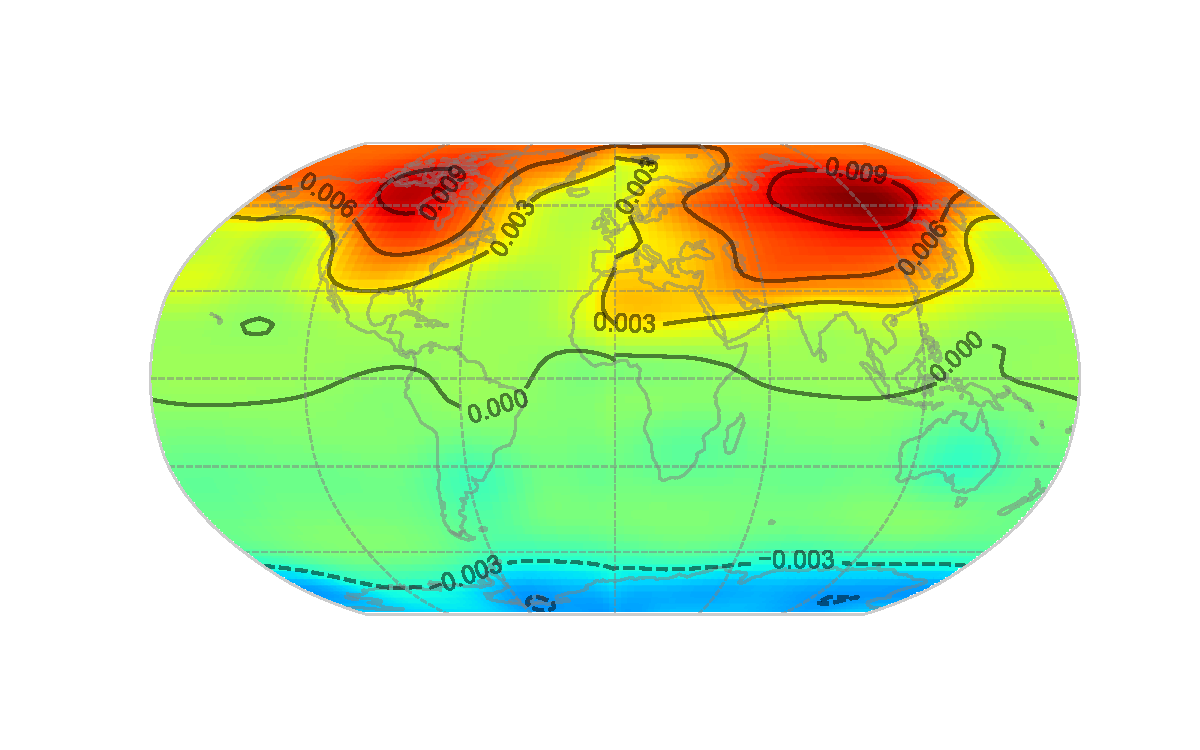
\includegraphics[width=\textwidth]{ftsm_res_TREFHT_fpc_0}
		\caption{$\vesub{\bar{\phi}}{1}$}
		\label{fig:ftsm_res_TREFHT_fpc_1}
	\end{subfigure}
	\vfill       
	\begin{subfigure}[b]{0.45\textwidth}
		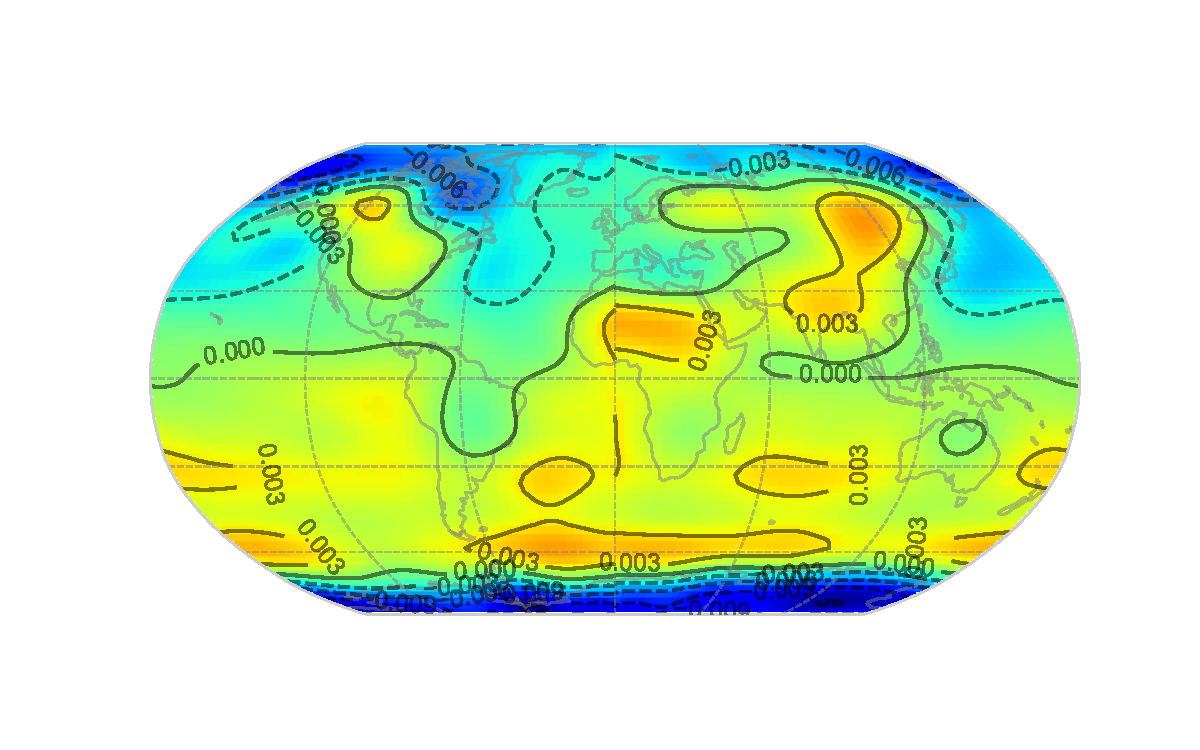
\includegraphics[width=\textwidth]{ftsm_res_TREFHT_fpc_1}
		\caption{$\vesub{\bar{\phi}}{2}$}
		\label{fig:ftsm_res_TREFHT_fpc_2}
	\end{subfigure}
	\begin{subfigure}[b]{0.45\textwidth}
		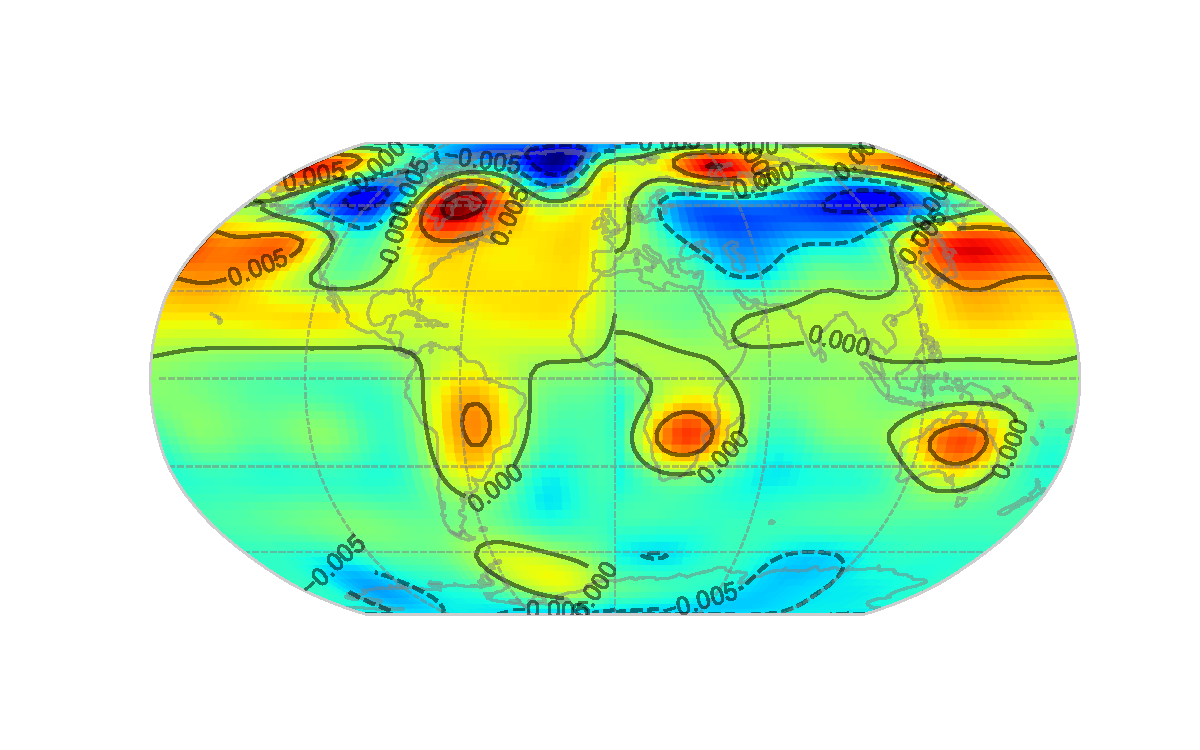
\includegraphics[width=\textwidth]{ftsm_res_TREFHT_fpc_2}
		\caption{$\vesub{\bar{\phi}}{3}$}
		\label{fig:ftsm_res_TREFHT_fpc_3}
	\end{subfigure}
	\caption[Example of the functional principal components generated by the FPCA model with the TREFHT variable of the CESM-LE dataset.]{Example of the functional principal components generated by the FPCA model with the TREFHT variable of the CESM-LE dataset. Notice how each component shows a different mode of spatial variation present in the process. Such decompositions like these can be useful to understanding the process as a whole.}
	\label{fig:ftsm_res_TREFHT_fpc}
\end{figure}

\begin{figure}
	\centering
	\begin{subfigure}[b]{0.45\textwidth}
		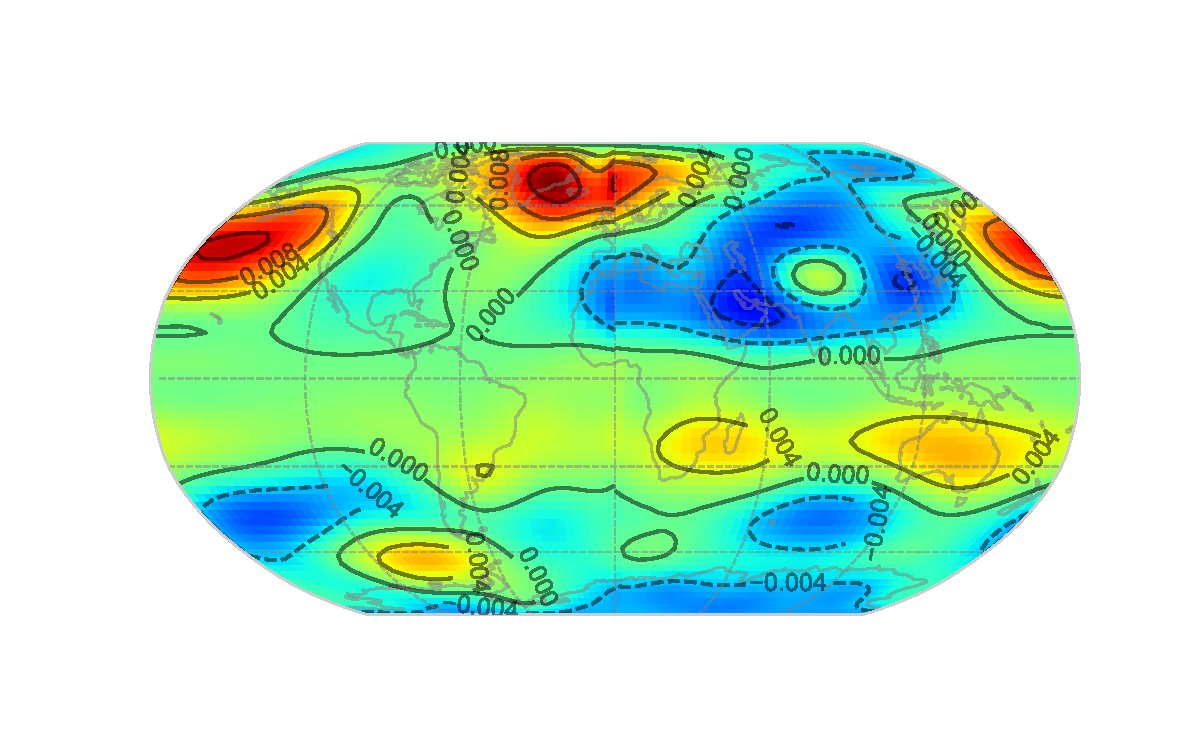
\includegraphics[width=\textwidth]{ftsm_res_PS_fpc_0}
		\caption{$\vesub{\bar{\phi}}{1}$}
		\label{fig:ftsm_res_PS_fpc_1}
	\end{subfigure}
	\vfill       
	\begin{subfigure}[b]{0.45\textwidth}
		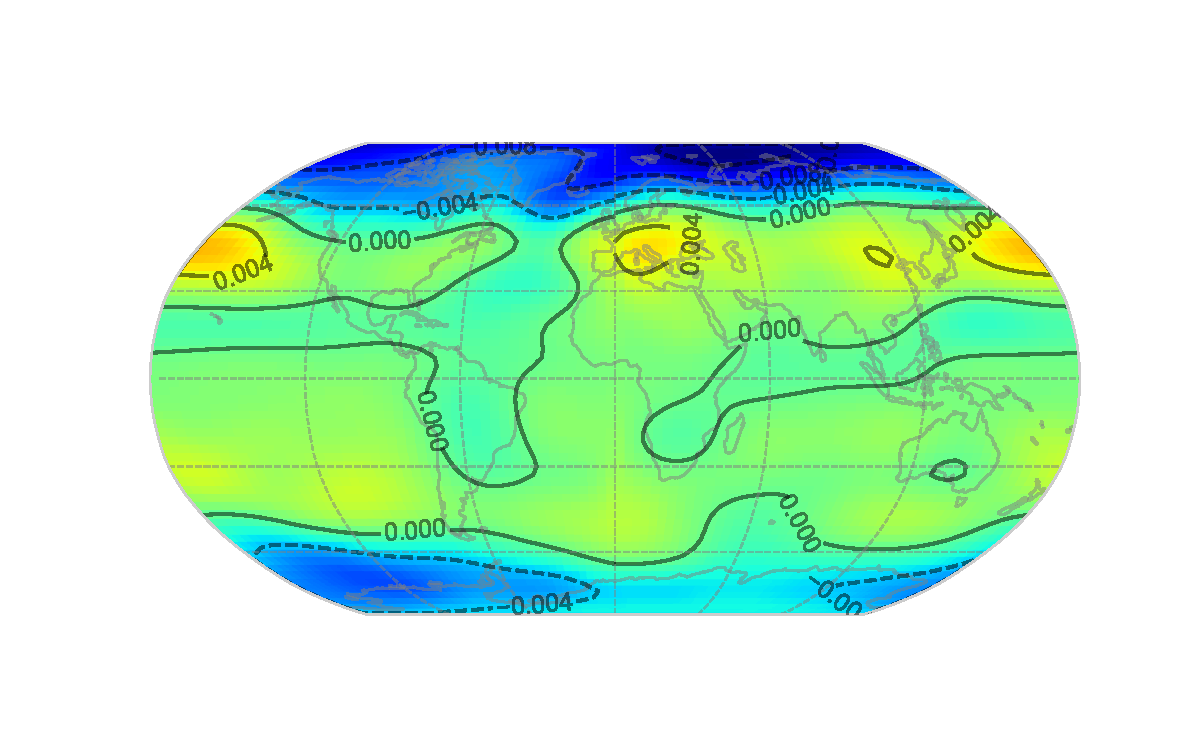
\includegraphics[width=\textwidth]{ftsm_res_PS_fpc_1}
		\caption{$\vesub{\bar{\phi}}{2}$}
		\label{fig:ftsm_res_PS_fpc_2}
	\end{subfigure}
	\begin{subfigure}[b]{0.45\textwidth}
		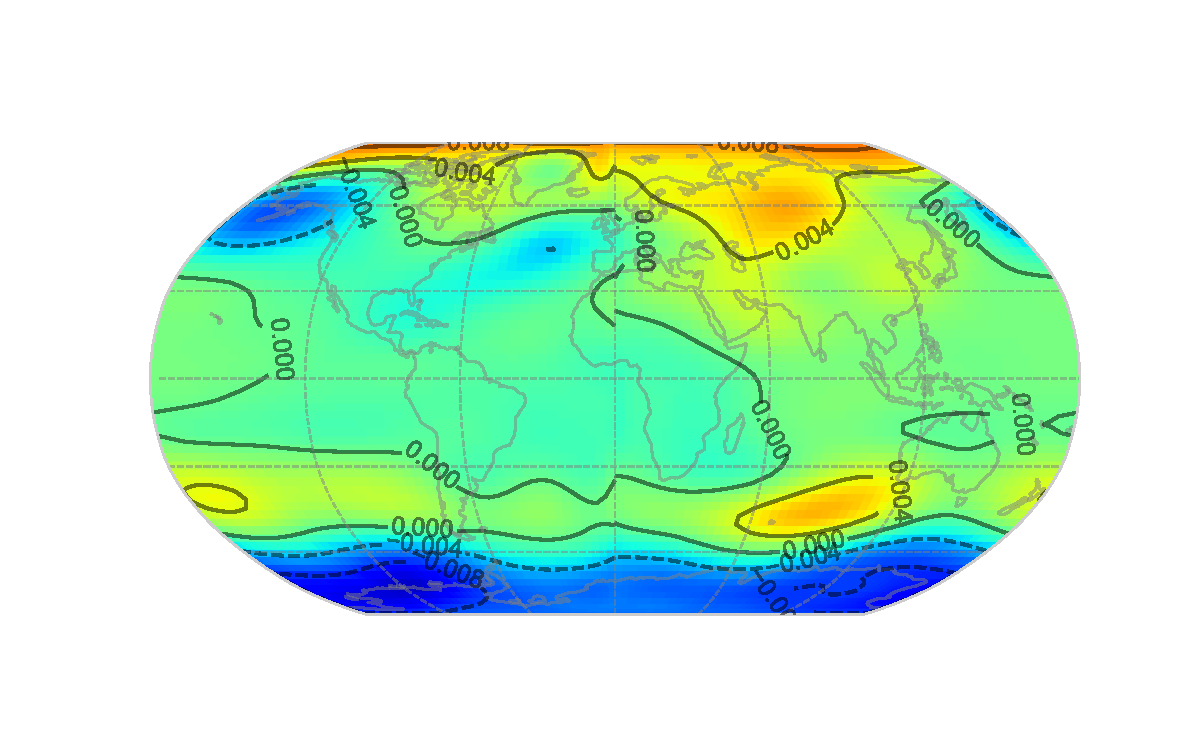
\includegraphics[width=\textwidth]{ftsm_res_PS_fpc_2}
		\caption{$\vesub{\bar{\phi}}{3}$}
		\label{fig:ftsm_res_PS_fpc_3}
	\end{subfigure}
	\caption[Example of the functional principal components generated by the FPCA model with the PS variable.]{Example of the functional principal components generated by the FPCA model with the PS variable of the CESM-LE data set. Notice how each component shows a different mode of spatial variation present in the process. Such decompositions like these can be useful to understanding the process as a whole.}
	\label{fig:ftsm_res_PS_fpc}
\end{figure}

The standard PACE methodology can be seen to do well on the real world EO data set due to its ability to capture small scale variations.
This occurs essentially because we treat each spatial location independently.
However, we have seen from both the FPCA and MAFR models that incorporating spatial information can be useful in recovering unobserved surfaces.
Utilising spatial dependency also has the added benefit of helping to ignore unstructured noise processes. 
A combination of both methodologies may then be desirable; that is to incorporate spatial information into the PACE model.
The challenge is then to do so in such a way that keeps the model performing well where there exists small scale spatial variation.
In the following chapters we consider such a model. 